%!TEX root =../quadrotorbook.tex
\chapter{Trajectory Generation and Local Planning}
\label{chap:trajectory_planning}

The objective of this chapter is to plan trajectories through a map that represents a cluttered world environment.  The high-level architecture for this chapter is shown in Figure~\ref{fig:planning_architecture}.
\begin{marginfigure}[3in]
  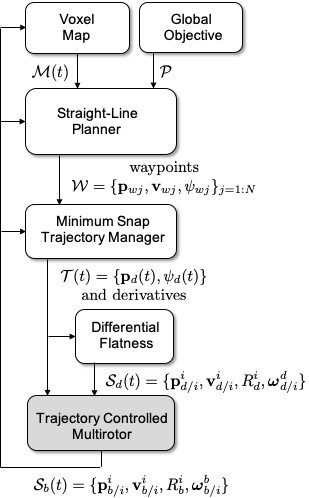
\includegraphics[width=\linewidth]{chap5_trajectory_planning/figures/planning_architecture}
  \caption{The path planning architecture outlined in this chapter.}
  \label{fig:planning_architecture}  
\end{marginfigure}
At the highest level is a voxel representation of the world, local the the multirotor.  The voxel grid will evolve dynamically so that the multirotor always remains in voxel at the center of the map.  A straight-line path planner is then used to plan paths through the voxel map that minimize the distance to the goal location as well as minimize the associated risk.  The output of the straight-line planner is a set of waypoints $\mathcal{W}$ specified as a sequence of desired positions, desired velocities, and desired heading directions.  The waypoints are processed by the {\em minimum-snap trajectory} block to produce a time trajectory of position and heading where the fourth derivative (snap) of the position trajectory is minimized.  The trajectory can be fed directly into the trajectory following framework discussed in Chapter~\ref{chap:trajectory_following}.  However, the framework in Chapter~\ref{chap:trajectory_following} also requires velocity, and angular velocity of the desired multirotor frame.  Those elements are naturally produced by the {\em differential flatness} block shown in Figure~\ref{fig:planning_architecture}.


%----------------------------------
\section{Differential Flatness}
\label{sec:differential_flatness}

Consider the nonlinear system
\begin{equation}\label{eq:flat-system}
\dot{x} = f(x,u),
\end{equation}
where $x$ is the state and $u\in\mathbb{R}^m$ is the control input, and the output mapping
\begin{equation}\label{eq:flat-output}
z = h(x),
\end{equation}
where $z\in\re^p$.  We say that the system~\eqref{eq:flat-system} is differentially flat with flat output $z$ if the following conditions hold~\cite{CowlingYakimenkoWhidborne07}:
\begin{enumerate}
\item The components of $z$ are not differentially related over time.
\item The states $x$ can be written as a function of the flat output and its derivatives, i.e., there exists a function $g_1$, and a finite scalar $m_1$ such that
    \begin{equation}\label{eq:flat-g1}
    x(t) = g_1\left(z(t),\frac{d}{dt}z(t),\cdots,\frac{d^{m_1}}{dt^{m_1}}z(t)\right).
    \end{equation}
\item The control inputs $u$ can be written as a function of the flat output and its derivatives, i.e., there exists a function $g_2$ and a finite scalar $m_2$ such that
    \begin{equation}\label{eq:flat-g2}
    u(t) = g_2\left(z(t),\frac{d}{dt}z(t),\cdots,\frac{d^{m_2}}{dt^{m_2}}z(t)\right).
    \end{equation}
\end{enumerate}

We now show that the multi-rotor system is differentially flat.

\begin{theorem}[Multirotor is Differentially Flat]

Suppose that the multirotor system is given by
\begin{align}
\dot{\pbf}_{d/i}^i &= \vbf_{d/i}^i \label{eq:flat-multirotor-1} \\
\dot{\vbf}_{d/i}^i &= g \ebf_3 + T_d R_d^i \ebf_3 \label{eq:flat-multirotor-2} \\
\dot{R}_d^i &= R_d^i \ss{\omegabf_{d/i}^d}, \label{eq:flat-multirotor-3}
\end{align}
and let $\psi$ be the heading angle, i.e., the body $x$-axis projected onto the inertial $x-y$ plane is 
$\sbf_\psi\doteq (\cos\psi, \sin\psi, 0)^\top$.  

Then the multirotor system is differentially flat with flat outputs $\{\pbf_d(t), \psi_d(t)\} \in\mathbb{R}^3 \times \mathbb{R}$.
\end{theorem}
\begin{proof}
To show that the system is differentially flat, the state variables $\pbf_{d/i}^i$, $\vbf_{d/i}^i$, $R_d^i$ and the input variables $T_d$ and $\omegabf_{d/i}^d$ must all be expressed in terms of the flat outputs $\{\pbf_d(t), \psi_d(t)\}$ and their derivatives.

The position states are directly expressed in the flat outputs as $\pbf_{d/i}^i = \pbf_d(t)$.  The velocity states are directly expressed in the derivative of the flat outputs as $\vbf_{d/i}^i = \dot{\pbf}_d(t)$.

Let the rotation matrix be expressed as 
\[
R_d^i = \begin{pmatrix} \rbf_{1d} & \rbf_{2d} & \rbf_{3d} \end{pmatrix},
\]
where $r_{jd}$ is the $j^{th}$ desired body axis of the multirotor expressed in the inertial frame. Therefore Equation~\eqref{eq:flat-multirotor-2} becomes
\[
T_d r_{3d} = \dot{\vbf}_{d/i}^i - g \ebf_3,
\]
which implies that 
\begin{align*}
T_d &= \norm{\dot{\vbf}_{d/i}^i - g \ebf_3^i} \\
\rbf_{3d} &= \frac{\dot{\vbf}_{d/i}^i - g \ebf_3}{\norm{\dot{\vbf}_{d/i}^i - g \ebf_3}}.
\end{align*}
Therefore the input $T_d$ and the third row of the rotation matrix can be expressed in terms of the flat output as
\begin{align*}
T_d &= \norm{\ddot{\pbf}_d - g \ebf_3} \\
\rbf_{3d} &= \frac{\ddot{\pbf}_d - g \ebf_3}{\norm{\ddot{\pbf}_d- g \ebf_3}}.
\end{align*}
The cross product between the body frame $z$-axis $\rbf_{3d}$ and the heading vector $\sbf_{\psi_d}$ will be in the direction of the body frame $y$-axis and should always be in the inertial $x-y$ plane.  Therefore, $\rbf_{2d}$ is expressed in terms of the flat outputs as
\[
\rbf_{2d} = \frac{\rbf_{3d} \times \sbf_{\psi_d}}{\norm{\rbf_{3d} \times \sbf_{\psi_d}}}.
\]
Since the body frame is a right-handed coordinate system, the body $x$-axis is given by
\[
\rbf_{1d} = \rbf_{2d} \times \rbf_{3d}.
\]
We have shown that $R_d^i$ can be expressed in terms of $\dot{\pbf}_d$ and $\psi_d$.  By differentiating $R_d^i$ it is clear that $\dot{R}_d^i$ can be expressed in terms of $\dot{\pbf}_d$, $\ddot{\pbf}_d$, $\psi_d$ and $\dot{\psi}_d$.  

From Equation~\eqref{eq:flat-multirotor-3}, the angular velocity vector is given by
\[
\omegabf_{d/i}^d = \left(R_d^{i\top} \dot{R}_d^i\right)^\vee. 
\]

Summarizing, the states and outputs are expressed in the flat outputs and their derivatives as
\begin{align}
\pbf_{d/i}^i(\pbf_d) &= \pbf_d(t) \notag \\
\vbf_{d/i}^i(\dot{\pbf}_d) &= \dot{\pbf}_d(t) \notag \\
\rbf_{3d}(\ddot{\pbf}_d) &= \frac{\ddot{\pbf}_d - g \ebf_3}{\norm{\ddot{\pbf}_d - g \ebf_3}} \notag \\
\rbf_{2d}(\ddot{\pbf}_d, \psi_d) &= \frac{\rbf_{3d} \times \sbf_{\psi_d}}{\norm{\rbf_{3d} \times \sbf_{\psi_d}}} \notag \\
\rbf_{1d}(\ddot{\pbf}_d, \psi_d) &= \rbf_{2d} \times \rbf_{3d} \label{eq:differential_flatness_equations} \\
R_d^i(\ddot{\pbf}_d, \psi_d) &= \begin{pmatrix} \rbf_{1d} & \rbf_{2d} & \rbf_{3d} \end{pmatrix} \notag \\
T_d(\ddot{\pbf}_d) &= \norm{\ddot{\pbf}_d - g \ebf_3} \notag \\	
\omegabf_{d/i}^d(\ddot{\pbf}_d, \dddot{\pbf}_d, \psi_d, \dot{\psi}_d) &= (R_d^{i\top}\dot{R}_d^i)^\vee.\notag 
\end{align}

Since all states and inputs can be expressed in terms of the flat outputs and their derivatives, the system is differentially flat.
\end{proof}

The inclusion of the induced drag term in the dynamics does not change the differential flatness property, although it does change equations expressions for the states and input variables.  The complete derivation is given in~\cite{FaesslerFranchiScaramuzza18.pdf}.


%\subsection{Differential Flatness of Quadrotor Dynamics Subject to Rotor Drag, RAL, 2018}
%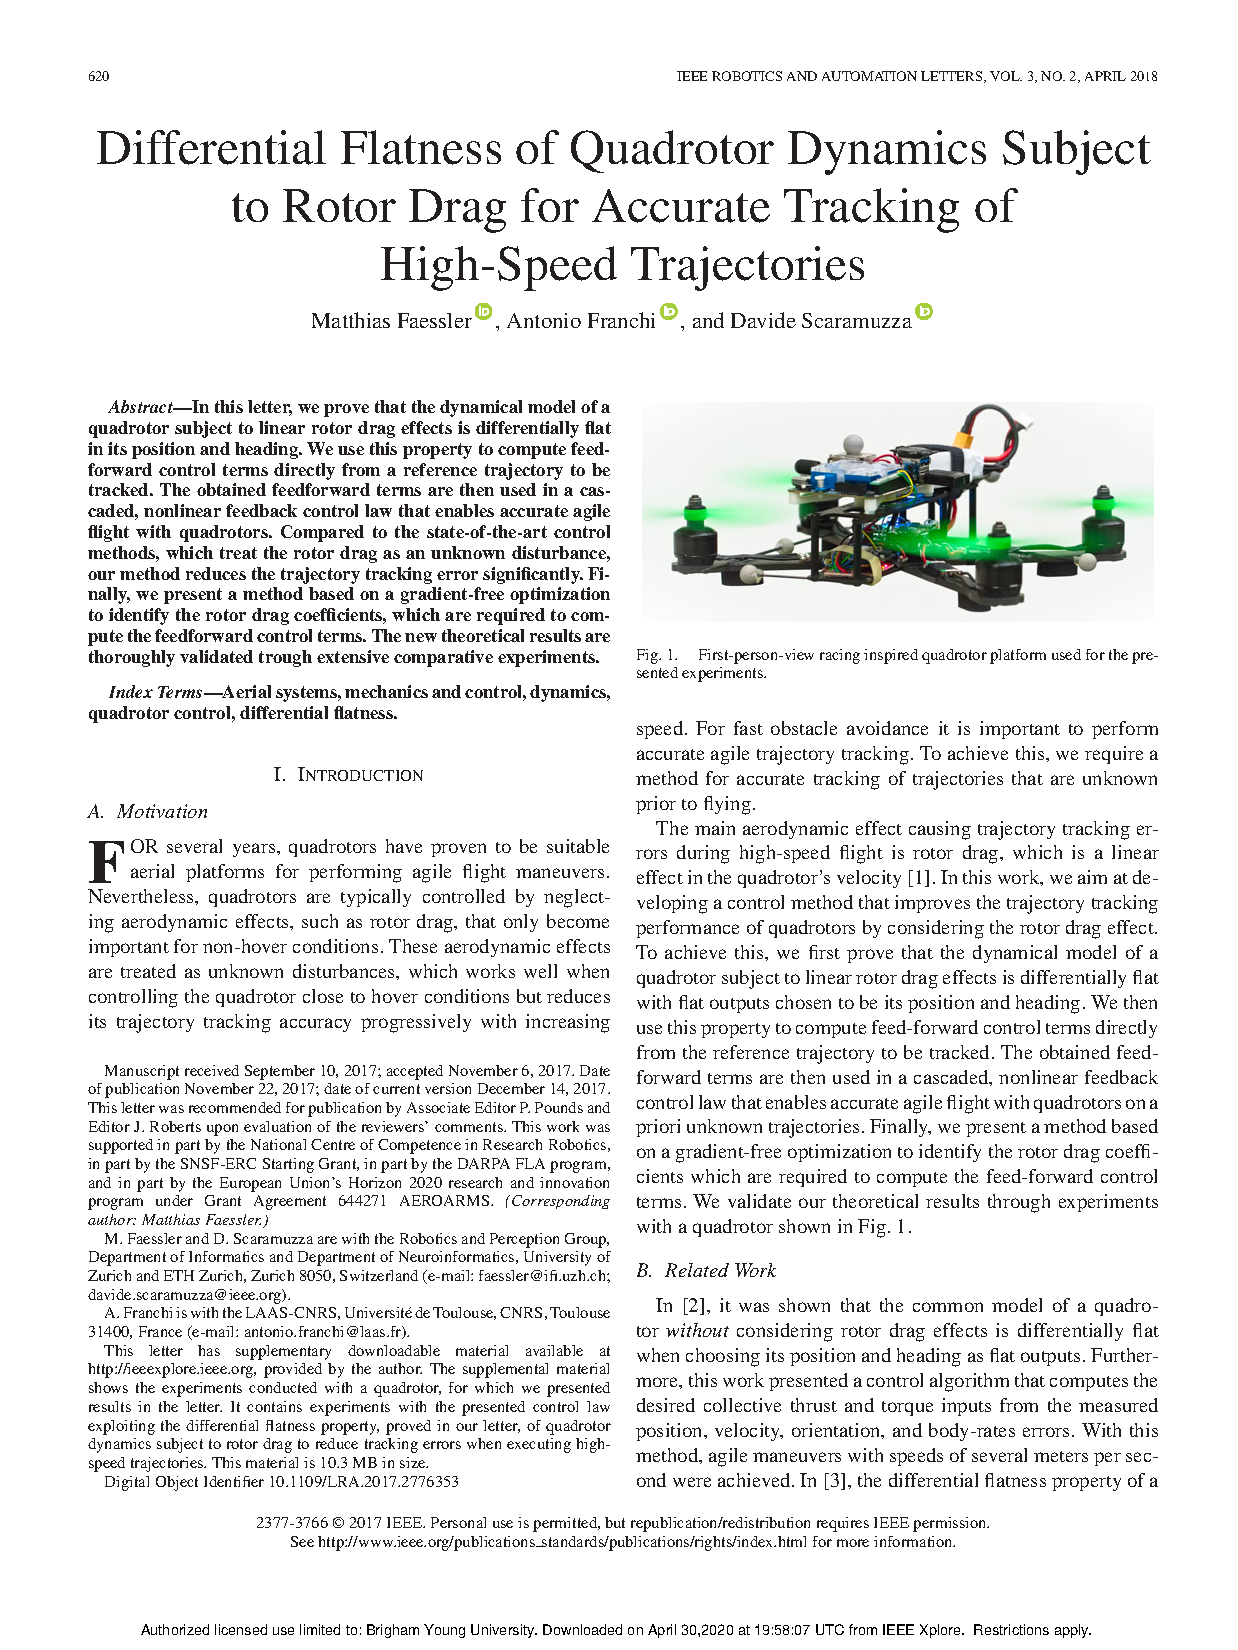
\includepdf[pages=-,scale=.8,pagecommand={}]{chap5_trajectory_planning/papers/FaesslerFranchiScaramuzza18.pdf}




%++++++++++++++++++++++++++++++++++++++++++++++++++++++++++++++
\subsection{Analytic calculation of desired angular velocity}
Author: Jacob Willis

%
%\usepackage[utf8]{inputenc}
%\usepackage{amsmath}
%\usepackage{amssymb}
%\usepackage{graphicx}
%\graphicspath{ {./figs/} }
%
%% \usepackage{theorem}
%\usepackage{amsthm}
%\newtheorem{theorem}{Theorem}
%\newtheorem{property}{Property}
%\def\proof{\hspace{1em}{\it Proof: }}
%\def\endproof{\hspace*{\fill}~$\blacksquare$\par\endtrivlist\unskip}
%
%\newtheorem*{remark}{Remark}
%
%\usepackage[hidelinks]{hyperref}
%\usepackage{color}
%\newcommand{\rwbcomment}[1]{{\color{red} RWB: #1}}
%\newcommand{\jbwcomment}[1]{{\color{blue} JBW: #1}}
%%\usepackage{cite}
%\usepackage{multirow}
%\usepackage[margin=1in]{geometry}
%
%\usepackage{biblatex}
%\addbibresource{bib_willis/references.bib}
%
%%\DeclareMathOperator{\mod}{mod}
%\DeclareMathOperator{\floor}{floor}
%\DeclareMathOperator{\rank}{rank}
%\DeclareMathOperator{\vspan}{span}
%\DeclareMathOperator*{\argmin}{arg min}
%
%\title{\LARGE Analytic Derivative of the Desired Rotation Matrix for Control}
%\author{Jacob Willis}
%
%\begin{document}
%\maketitle

Rather than numerically differentiating $R_d^i$ as described in Section~\ref{sec:numerical_differentiation_of_R}, this section shows how to find the time derivative of $R_d^i$ analytically.
First, recall that
\begin{equation}
	R_d^i = \begin{pmatrix} \mathbf{r}_{1d} & \mathbf{r}_{2d}&  \mathbf{r}_{3d} \end{pmatrix}
\end{equation}
and therefore that
\begin{equation}
	\dot{R}_d^i = \begin{pmatrix} \dot{\mathbf{r}}_{1d} & \dot{\mathbf{r}}_{2d} & \dot{\mathbf{r}}_{3d} \end{pmatrix}.
\end{equation}

To proceed, we need the following two properties.
\begin{property}
	The time derivative of the cross product of two time-dependent vectors $\mathbf{x}$ and $\mathbf{y}$ is
	\begin{equation}
		\label{eq:cross_derivative}
		\frac{d}{dt} (\mathbf{x} \times \mathbf{y}) = \dot{\mathbf{x}} \times \mathbf{y} + \mathbf{x} \times \dot{\mathbf{y}}
	\end{equation}
\end{property}
\proof
This is easiest to see by recalling that $\mathbf{x} \times \mathbf{y} = \mathbf{x}^\wedge \mathbf{y}$ where the result follows from the product rule.
\endproof

\begin{property} \label{prop:derivative_of_normal_vector}
	The time derivative of a normalized vector $\frac{\mathbf{x}}{\|\mathbf{x}\|}$ is
	\begin{equation}
		\label{eq:norm_derivative}
		\frac{d}{dt} \left(\frac{\xbf}{\norm{\xbf}}\right) = \Pi_{\frac{\xbf}{\norm{\xbf}}} \frac{\dot{\xbf}}{\norm{\xbf}},
	\end{equation}
	where $\Pi_{\nbf} \doteq I-\nbf\nbf^\top$ is the projection operator on to the plane orthogonal to the unit vector $\nbf$.
\end{property}
\proof
	By the quotient rule, we have
	\begin{equation}
		\frac{d}{dt} \frac{\mathbf{x}}{\|\mathbf{x}\|} = \frac{\dot{\mathbf{x}} \|\mathbf{x}\| - \mathbf{x} \frac{d}{dt}(\|\mathbf{x}\|)}{\|\mathbf{x}\|^2}.
	\end{equation}
	Now,
	\begin{align}
		\frac{d}{dt} \|\mathbf{x}\| 
		= \frac{d}{dt} \sqrt{\mathbf{x}^\top \mathbf{x}} 
		= \frac{1}{2 \sqrt{\mathbf{x}^\top \mathbf{x}}} (\dot{\mathbf{x}}^\top \mathbf{x} + \mathbf{x}^\top \dot{\mathbf{x}})
		= \frac{\dot{\mathbf{x}}^\top \mathbf{x}}{\|\mathbf{x}\|}
	\end{align}
	Plugging in, we get
	\begin{equation}
		\frac{d}{dt} \frac{\mathbf{x}}{\|\mathbf{x}\|} = \frac{\dot{\mathbf{x}}}{\|\mathbf{x}\|} - \mathbf{x} \frac{\dot{\mathbf{x}}^\top \mathbf{x}}{\|\mathbf{x}\|^3}.
	\end{equation}
	Rearranging gives
	\[
	\frac{d}{dt} \frac{\mathbf{x}}{\|\mathbf{x}\|} =  \left(I-\frac{\xbf}{\norm{\xbf}}\frac{\xbf^\top}{\norm{\xbf}}\right)\frac{\dot{\xbf}}{\norm{\xbf}}.
	\]

\endproof

The third column of the rotation matrix is given by
\begin{equation}
	\mathbf{r}_{3d} = - \frac{\ddot{\mathbf{p}}_d - g \mathbf{e}_3 - K_p \tilde{\mathbf{p}} - K_d \dot{\tilde{\mathbf{p}}}} {\norm{\ddot{\pbf}_d - g \ebf_3 - K_p \tilde{\pbf} - K_d \dot{\tilde{\pbf}}}}.
\end{equation}
Therefore, using the properties above we get that
\[
\dot{\rbf}_{3d} = \Pi_{\rbf_{3d}} \left(\frac{-\dddot{\pbf}_d + K_p \dot{\tilde{\pbf}} + K_d \ddot{\tilde{\pbf}}}{\norm{\ddot{\pbf}_d - g \ebf_3 - K_p \tilde{\pbf} - K_d \dot{\tilde{\pbf}}}}\right).
\]
The second column of the rotation matrix is given by
\[
\rbf_{2d} = \frac{\rbf_{3d}\times\sbf_{\psi_d}}{\norm{\rbf_{3d}\times\sbf_{\psi_d}}},
\]
which implies that
\[
\dot{\rbf}_{2d} = \Pi_{\rbf_{2d}}\left(\frac{\dot{\rbf}_{3d}\times\sbf_{\psi_d}+\dot{\psi}_d\rbf_{3d}\times (-\sin\psi_d,  \cos\psi_d, 0)^\top }{\norm{\rbf_{3d}\times\sbf_{\psi_d}}}\right).
\]
The first column of the rotation matrix is given by
\[
\rbf_{1d} = \rbf_{2d}\times\rbf_{3d},
\]
which implies that
\[
\dot{\rbf}_{1d} = \dot{\rbf}_{2d}\times\rbf_{3d} + \rbf_{2d}\times \dot{\rbf}_{3d}.
\]
The angular velocity can now be calculated as
\[
\omegabf_{d/i}^d(\pbf_d, \dot{\pbf}_d, \ddot{\pbf}_d, \dddot{\pbf}_d, \psi_d, \dot{\psi}_d) = \left[\begin{pmatrix}\rbf_{1d} & \rbf_{2d} & \rbf_{3d}\end{pmatrix}^\top \begin{pmatrix} \dot{\rbf}_{1d} & \dot{\rbf}_{2d} & \dot{\rbf}_{3d} \end{pmatrix}\right]^\vee.
\]





%----------------------------------
\section{An Introduction to B-Spline}


The objective of these notes is to explore spline methods for robotic applications. In general, the position of a robot in Euclidian space can be described by a time parametrized trajectory $\mathbf{p}(t)\in\mathbb{R}^3$, $t\in[a,b]$.  The time parametrized trajectory can be parameterized using a weighted sum of basis function as
\[
\mathbf{p}(t) = \sum_{m=0}^{N-1} \cbf_m \phi_m(t),
\]
where $\cbf_m\in\mathbb{R}^n$, and $\phi_m(t)$ are a set of basis functions.  For example, the basis functions could be the set of polynomial power function $\phi_m(t) = t^{m}/{m}|!$, or the set of sinusoidal function $\phi_m(t) = \sin(\frac{2\pi {m}}{N}t)$.  The disadvantage of both the polynomial power functions and sinusoidal functions is that the basis functions are defined for all $t\in[a,b]$ and so each control points $\mathbf{c}_m$ influences the entire trajectory.  Another disadvantage is that a large number of basis functions may be required to represent complicated trajectories.  

In these notes, we will use B-spline basis functions which have a number of very nice properties that we will explore.  In particular, a {\em B-spline} trajectory has the following form
\begin{equation}\label{eq:general-b-spline}
\mathbf{p}(t) = \sum_{m=0}^{M+d-1} \cbf_m b_m^d(t, \mathbf{t}),
\end{equation}
where $\cbf_m\in\mathbb{R}^n$ are the control points,  $\mathbf{t}=(\tau_0, \tau_1, \tau_2, \dots, \tau_T)$ are called the knot points where $i<j \implies \tau_i\leq \tau_j$, and $b_m^d(t, \mathbf{t})$ are the B-spline basis functions of degree $d$, given the knot sequence $\mathbf{t}$. The spline trajectories will be defined for $t$ in the interval, i.e., $t\in[\tau_d, \tau_{d+M}]$, which we will write as $t\in\text{span}(\mathbf{t})$

%Section~\ref{sec:b-spline-basis-functions} defines the B-spline basis function $b_m^d(t,  \mathbf{t})$ and describes some of their properties that will be useful for path planning and for estimation.
%Section~...
%% overview of other sections

%---------------------------------------------------------------
\subsection{B-Spline Basis Functions}
\label{sec:b-spline-basis-functions}

The B-spline basis function are defined by the recursive formula:
\begin{align}
b_m^0(t, \mathbf{t}) &= \begin{cases} 1 & \text{~if~} \tau_m \leq t \leq \tau_{m+1} \\ 
 									 0 & \text{~otherwise} 
 					   \end{cases} 
	\label{eq:spline_basis_definition_0}\\	
b_m^d(t, \mathbf{t}) &= w_m^d(t, \mathbf{t}) b_m^{d-1}(t, \mathbf{t}) + \left[1-w_{m+1}^d(t, \mathbf{t})\right] b_{m+1}^{d-1}(t,  \mathbf{t}),
	\label{eq:spline_basis_definition_k} \\
w_m^d(t, \mathbf{t}) &= \begin{cases}
                      		\frac{t-\tau_m}{\tau_{m+d}-\tau_m}, & \tau_{m+d}\neq \tau_m \\
                      		0, & \text{~otherwise} 
                        \end{cases}.
     \label{eq:spline_basis_definition_w}
\end{align}

%+++++++++++++++++++++++++++++++
\par\noindent{\bf Zero degree basis}

For example, if the knot vector is given by
\[
\mathbf{t} = [\tau_0, \tau_1, \tau_2] \defeq [0, 1, 2],
\]
then there are two basis function of degree $d=0$ given by
\begin{align*}
b_0^0(t,\mathbf{t}) &= \begin{cases} 1 & \text{~if~} \tau_0 \leq t \leq \tau_1 \\ 
 									 0 & \text{~otherwise} 
 			\end{cases}
\\ 
b_1^0(t,\mathbf{t}) &= \begin{cases} 1 & \text{~if~} \tau_1 \leq t \leq \tau_2 \\ 
 									 0 & \text{~otherwise}
 			\end{cases}
\end{align*}
where $b_0^1(t,\mathbf{t})$ and $b_1^0(t,\mathbf{t})$ are shown in Figure~\ref{fig:spline_basis_0}.
\begin{marginfigure}[0in]
  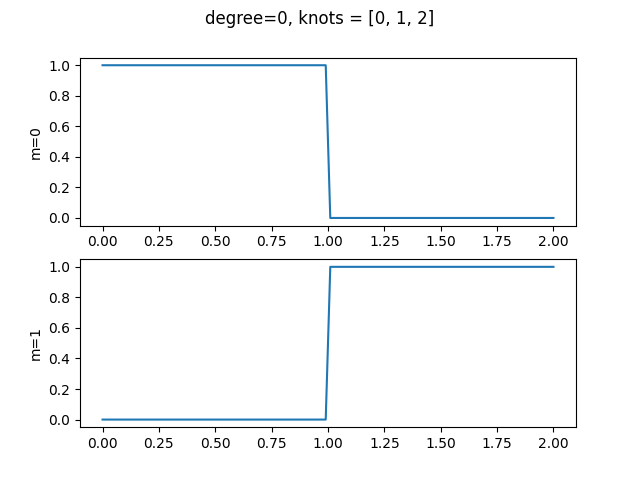
\includegraphics[width=\linewidth]{./chap5_trajectory_planning/figures/spline_basis_0}
  \caption{Zeros degree spline basis}
  \label{fig:spline_basis_0}  
\end{marginfigure}
Note that $b_1^0(t,\mathbf{t}) = b_0^0(t-1,\mathbf{t})$, or in other words, all zero degree basis functions are shifted versions of the central zero degree basis function $b_0^0(t,  \mathbf{t})$.  Additional zero degree basis function can be defined by expanding the knot vector to $\mathbf{t}=[0, \dots, M]$, where $b_m^0(t,  \mathbf{t})= b_0^0(t-m; \mathbf{t})$ for $m\leq M$.


\clearpage


%+++++++++++++++++++++++++++++++
\par\noindent{\bf First degree basis}

If the knot vector is given by
\[
\mathbf{t} = [\tau_0, \tau_1, \tau_2, \tau_3, \tau_4] \defeq [0, 0, 1, 2, 2],
\]
then there are $2d+1=3$ unique basis function of degree $d=1$ given by
\begin{align*}
b_0^1(t,  \mathbf{t}) &= \frac{t-\tau_0}{\tau_1-\tau_0} b_0^0(t, \mathbf{t}) + \frac{\tau_2-t}{\tau_2-\tau_1}b_1^0(t,  \mathbf{t}) 
	= \begin{cases} 0   & \text{~if~} t_0=0 \leq t \leq t_1=0 \\
				    1-t & \text{~if~} t_1=0 \leq t \leq t_2=1 \\ 
 	  \end{cases}
\\ 
b_1^1(t,  \mathbf{t}) &= \frac{t-\tau_1}{\tau_2-\tau_1} b_1^0(t, \mathbf{t}) + \frac{\tau_3-t}{\tau_3-\tau_2}b_2^0(t,  \mathbf{t})
	= \begin{cases} t & \text{~if~} t_1=0 \leq t \leq t_2=1 \\ 
 									2-t & t_2=1 \leq t \leq t_3=2 \\
 									0 & \text{~otherwise}
 					    \end{cases}
\\ 
b_2^1(t,  \mathbf{t}) &= \frac{t-\tau_2}{\tau_3-\tau_2} b_2^0(t, \mathbf{t}) + \frac{\tau_4-t}{\tau_4-\tau_3}b_3^0(t,  \mathbf{t})
	= \begin{cases} t-1 & \text{~if~} t_2=1 \leq t \leq t_3=2 \\ 
 					0 & \text{~if~} t_3=2 \leq t \leq t_4=2 \\
 	  \end{cases}
\end{align*}
where $b_0^1(t,  \mathbf{t})$, $b_1^1(t,  \mathbf{t})$, and $b_2^1(t,  \mathbf{t})$ are shown on the left in Figure~\ref{fig:spline_basis_1}.
\begin{marginfigure}[-2in]
  	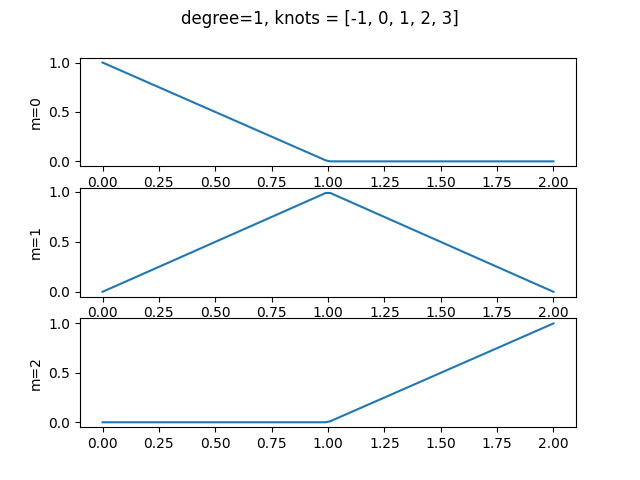
\includegraphics[width=\linewidth]{./chap5_trajectory_planning/figures/spline_basis_1}
  \caption{Degree one spline basis}
  \label{fig:spline_basis_1}  
\end{marginfigure}
\begin{marginfigure}[0in]
  	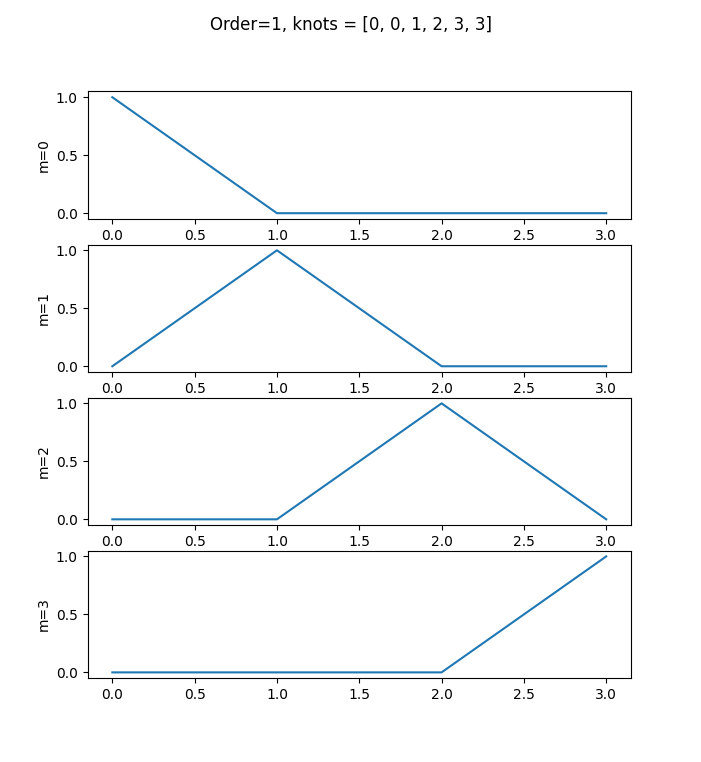
\includegraphics[width=\linewidth]{./chap5_trajectory_planning/figures/spline_basis_1_extra_knot}
  \caption{Degree one spline basis}
  \label{fig:spline_basis_1_extra_knot}  
\end{marginfigure}
If the knot vector is expanded by one time unit to
\[
\mathbf{t}' = [\tau_0, \tau_1, \tau_2, \tau_3, \tau_4, \tau_5] \defeq [0, 0, 1, 2, 3, 3],
\]
then there are still only three unique basis vectors, but 
$b_2^1(t,  \mathbf{t}')$ is a shifted version $b_1^1(t,  \mathbf{t})$ and $b_3^1(t,  \mathbf{t}')$ is a shifted version $b_2^1(t,  \mathbf{t})$, as shown on the right in Figure~\ref{fig:spline_basis_1}.

\clearpage


%+++++++++++++++++++++++++++++++
\par\noindent{\bf Second degree basis}

If the knot vector is given by
\[
\mathbf{t} = [\tau_0, \tau_1, \tau_2, \tau_3, \tau_4, \tau_5, \tau_6, \tau_7, \tau_8] \defeq [0, 0, 0, 1, 2, 3, 3, 3],
\]
then there are $2d+1=5$ unique basis function of degree $d=2$ given by
\begin{align*}
b_0^2(t,  \mathbf{t}) &= \frac{t-\tau_0}{\tau_2-\tau_0} b_0^1(t, \mathbf{t}) + \frac{\tau_3-t}{\tau_3-\tau_1}b_1^1(t,  \mathbf{t}) 
	= \begin{cases} (1-t)^2   & \text{~if~} 0 \leq t \leq 1 \\
				    0 & \text{~otherwise~}  \\ 
 	  \end{cases}
\\ 
b_1^2(t,  \mathbf{t}) &= \frac{t-\tau_1}{\tau_3-\tau_1} b_1^1(t, \mathbf{t}) + \frac{\tau_4-t}{\tau_4-\tau_2}b_2^1(t,  \mathbf{t})
	= \begin{cases} t(2-\frac{3}{2}t) & \text{~if~} 0 \leq t \leq 1 \\ 
 									\frac{(2-t)^2}{2} & 1 \leq t \leq 2 \\
 									0 & \text{~otherwise}
 					    \end{cases}
\\ 
b_2^2(t,  \mathbf{t}) &= \frac{t-\tau_2}{\tau_4-\tau_2} b_2^1(t, \mathbf{t}) + \frac{\tau_5-t}{\tau_5-\tau_3}b_3^1(t,  \mathbf{t})
	= \begin{cases} \frac{t^2}{2} & \text{~if~} 0 \leq t \leq 1 \\ 
 					-\frac{3}{2}t^2 + \frac{7}{2}t - \frac{3}{2} & \text{~if~} 1 \leq t \leq 2 \\
 					\frac{(3-t)^2}{2} & \text{~if~} 2 \leq t \leq 3 \\
 					0 & \text{~otherwise}
 	  \end{cases}
\\ 
b_3^2(t,  \mathbf{t}) &= \frac{t-\tau_2}{\tau_4-\tau_2} b_2^1(t, \mathbf{t}) + \frac{\tau_5-t}{\tau_5-\tau_3}b_3^1(t,  \mathbf{t})
	= \begin{cases} \frac{(t-1)^2}{2} & \text{~if~} 1 \leq t \leq 2 \\ 
 					-\frac{3}{2}t^2 + \frac{15}{2}t-\frac{15}{2} & \text{~if~} 2 \leq t \leq 3 \\
 					0 & \text{~otherwise}
 	  \end{cases}
\\ 
b_4^2(t,  \mathbf{t}) &= \frac{t-\tau_2}{\tau_4-\tau_2} b_2^1(t, \mathbf{t}) + \frac{\tau_5-t}{\tau_5-\tau_3}b_3^1(t,  \mathbf{t})
	= \begin{cases} (t-2)^2 & \text{~if~} 2 \leq t \leq 3 \\ 
 					0 & \text{~otherwise}
 	  \end{cases}.	   	  
\end{align*}
The unique second degree basis function are shown on the left in Figure~\ref{fig:spline_basis_2}.
\begin{marginfigure}[-8in]
  	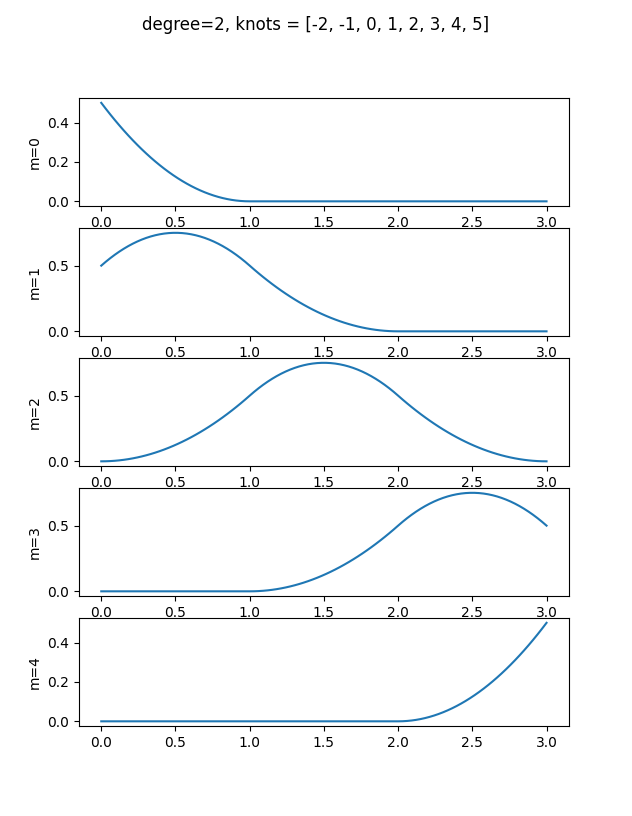
\includegraphics[width=\linewidth]{./chap5_trajectory_planning/figures/spline_basis_2}
  \caption{Second degree spline basis.}
  \label{fig:spline_basis_2}  
\end{marginfigure}
\begin{marginfigure}[-2.5in]
  	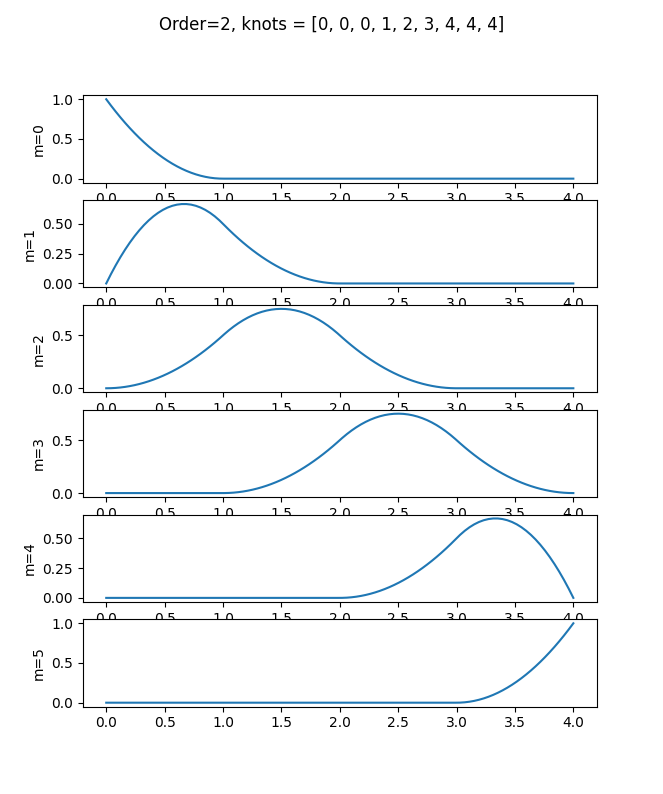
\includegraphics[width=\linewidth]{./chap5_trajectory_planning/figures/spline_basis_2_extra_knot}
  \caption{Second degree spline basis with extra knot}
  \label{fig:spline_basis_2}  
\end{marginfigure}
Expanding the knot vector by one time unit to 
\[
\mathbf{t}' = [\tau_0, \tau_1, \tau_2, \tau_3, \tau_4, \tau_5] \defeq [0, 0, 0, 1, 2, 3, 4, 4, 4],
\]
still results in $2d+1$ unique basis vectors, but $b_3^2(t,  \mathbf{t}')$ is a right-shifted version of $b_2^2(t,  \mathbf{t})$, and $b_4^2(t,  \mathbf{t}')$ and $b_5^2(t,  \mathbf{t})$ are a right-shifted versions of $b_3^2(t,  \mathbf{t}')$ and $b_4^2(t,  \mathbf{t})$, as shown on the right in Figure~\ref{fig:spline_basis_2}.

Similarly, the unique fourth order and ninth order basis functions are shown in Figures~\ref{fig:spline_basis_3} and~\ref{fig:spline_basis_8} respectively.

\begin{marginfigure}[0in]
  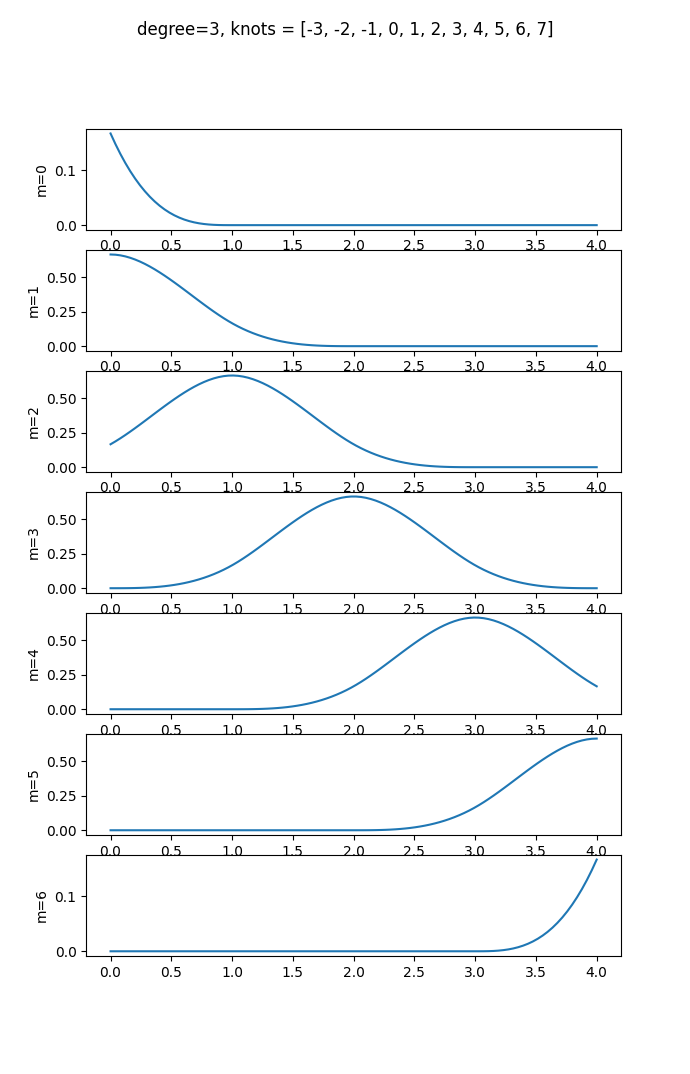
\includegraphics[width=\linewidth]{./chap5_trajectory_planning/figures/spline_basis_3}
  \caption{Third degree spline basis}
  \label{fig:spline_basis_3}  
\end{marginfigure}

\begin{figure}[ht]
  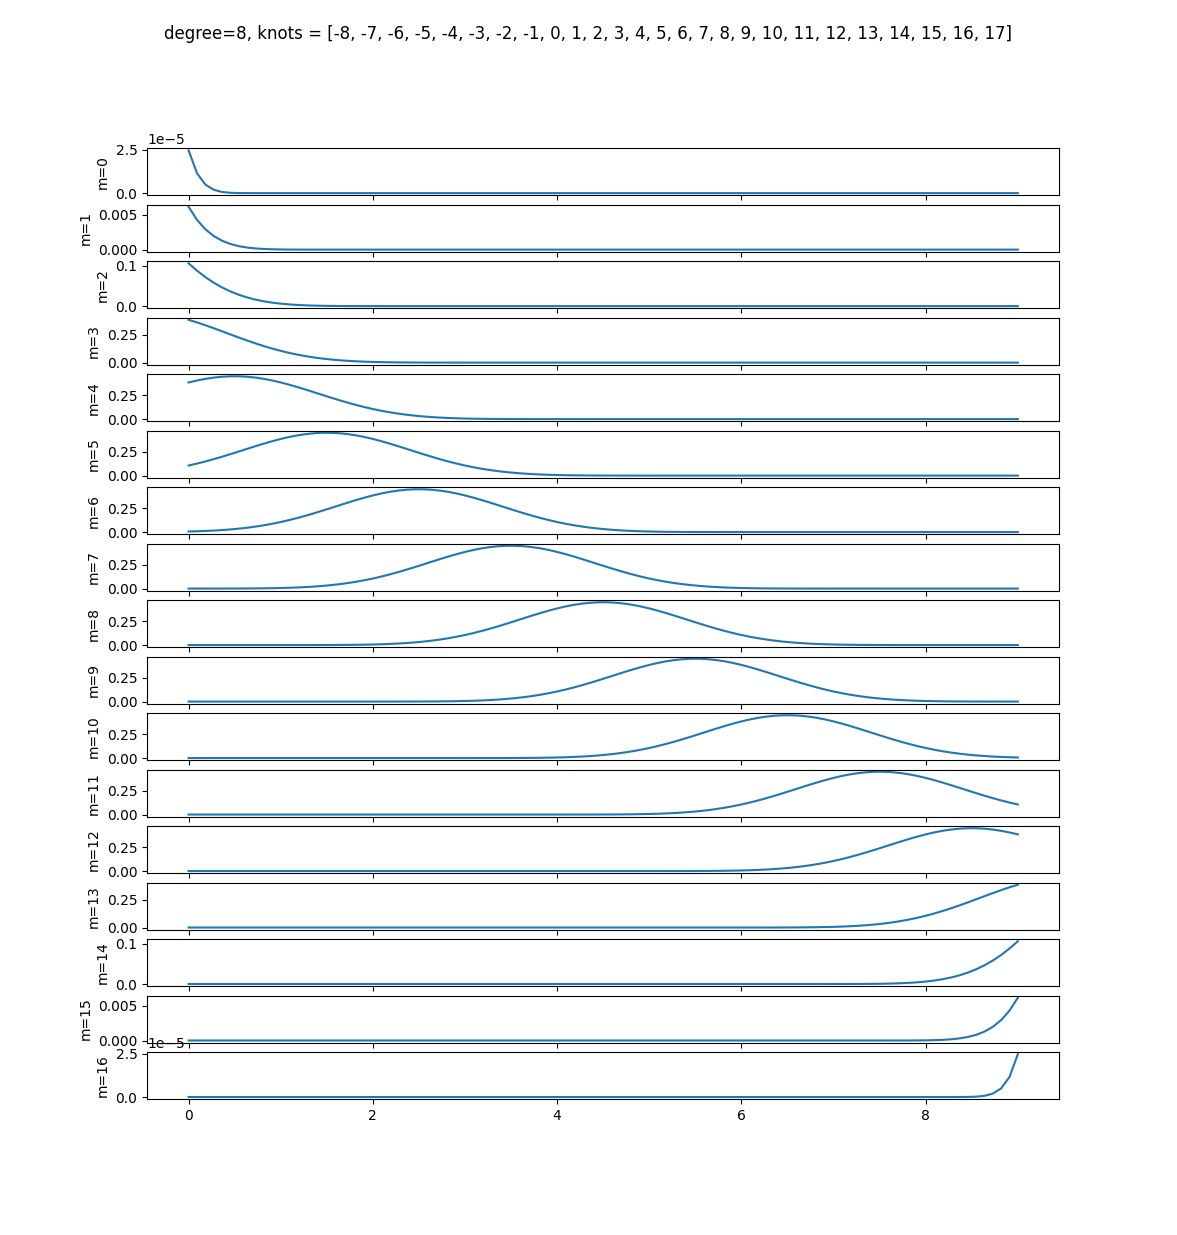
\includegraphics[width=\linewidth]{./chap5_trajectory_planning/figures/spline_basis_8}
  \caption{Eight degree spline basis}
  \label{fig:spline_basis_8}  
\end{figure}

\clearpage

%---------------------------------------------------------------
\par\noindent{\bf Shift and Scale Invariance of the Knot Sequence}

\begin{lemma} \label{lem:basis_are_shift_invariant}
Given an arbitrary knot sequence
\[
\mathbf{t} = [\tau_0, \tau_1, \dots \tau_T],
\]
an arbitrary time shift $\Delta$, and the one-sequence $\mathbf{1}\defeq[1, 1, \dots, 1]$, the B-spline basis functions are shift invariant in the sense that
if 
\[
\mathbf{t} + \Delta\mathbf{1} = [\tau_0+\Delta, \tau_1+\Delta, \dots \tau_T+\Delta]
\]
then
\[
b_j^d(t,  \mathbf{t}+\Delta\mathbf{1}) = b_j^d(t-\Delta, \mathbf{t}),
\]
i.e., shifting the knot sequence forward in time is identical to shifting the original B-spline forward in time.
\end{lemma}
\begin{proof}
When the degree is $d=0$, then equation~\eqref{eq:spline_basis_definition_0} gives
\begin{align*}
	b_j^0(t,  \mathbf{t}+\Delta\mathbf{1}) 
		&= \begin{cases} 1 & \text{~if~} \tau_j+\Delta \leq t \leq \tau_{j+1}+\Delta \\ 
 						 0 & \text{~otherwise} 
 		   \end{cases} \\
 		&= \begin{cases} 1 & \text{~if~} \tau_j \leq t-\Delta \leq \tau_{j+1} \\ 
 						 0 & \text{~otherwise} 
 		    \end{cases} \\ 	
 		&= b_j^0(t-\Delta, \mathbf{t}).
\end{align*}
Assuming that the statement holds when the order is $d\geq 1$, we get from 
Equation~\eqref{eq:spline_basis_definition_k} that
\begin{align*}
b_j^d(t,  \mathbf{t}+\Delta\mathbf{1}) &= \frac{t-\tau_j-\Delta}{\tau_{j+d}+\Delta-
\tau_j-\Delta} b_j^{d-1}(t,  \mathbf{t}+\Delta\mathbf{1}) + \frac{\tau_{j+d+1}+\Delta-t}{\tau_{j+d+1}+\Delta-\tau_{j+1}-\Delta} b_{j+1}^{d-1}(t,  \mathbf{t}+\Delta\mathbf{1}) \\
&= \frac{(t-\Delta)-\tau_j}{\tau_{j+d}-
\tau_j} b_j^{d-1}(t-\Delta, \mathbf{t}) + \frac{\tau_{j+d+1}-(t-\Delta)}{\tau_{j+d+1}-\tau_{j+1}} b_{j+1}^{d-1}(t-\Delta, \mathbf{t}) \\
&= b_j^d(t-\Delta, \mathbf{t}).
\end{align*}
The proof therefore follows by induction.
\end{proof}


\begin{lemma}\label{lem:bases_are_scale_invariant}
Given an arbitrary knot sequence
\[
\mathbf{t} = [\tau_0, \tau_1, \dots \tau_T]
\]
and an arbitrary scaling constant $\alpha\in\mathbb{R}$, the B-spline basis functions are scale invariant in the sense that
if 
\[
\alpha\mathbf{t} = [\alpha\tau_0, \alpha\tau_1, \dots \alpha\tau_T]
\]
then
\[
b_j^d(t,  \alpha\mathbf{t}) = b_j^d(t/\alpha, \mathbf{t}),
\]
i.e., scaling the knot sequence by $\alpha$ is identical to time scaling the original B-spline by $\frac{1}{\alpha}$.
\end{lemma}
\begin{proof}
When the degree is $d=0$, then equation~\eqref{eq:spline_basis_definition_0} gives
\begin{align*}
	b_j^0(t,  \alpha\mathbf{t}) 
		&= \begin{cases} 1 & \text{~if~} \alpha\tau_j \leq t \leq \alpha\tau_{j+1} \\ 
 						 0 & \text{~otherwise} 
 			\end{cases} \\
 		&= \begin{cases} 1 & \text{~if~} \tau_j \leq \frac{t}{\alpha} \leq \tau_{j+1} \\ 
 						 0 & \text{~otherwise} 
 			\end{cases} \\ 	
 		&= b_j^0(t/\alpha, \mathbf{t}).
\end{align*}
Assuming that the statement holds when the degree is $d\geq 1$, we get from 
Equation~\eqref{eq:spline_basis_definition_k} that
\begin{align*}
b_j^d(t,  \alpha\mathbf{t}) &= \frac{t-\alpha\tau_j}{\alpha\tau_{j+d}-
\alpha\tau_j} b_j^{d-1}(t,  \alpha\mathbf{t}) + \frac{\alpha\tau_{j+d+1}-t}{\alpha\tau_{j+d+1}-\alpha\tau_{j+1}} b_{j+1}^{d-1}(t,  \alpha\mathbf{t}) \\
&= \frac{(t/\alpha)-\tau_j}{\tau_{j+d}-
\tau_j} b_j^{d-1}(t/\alpha, \mathbf{t}) + \frac{\tau_{j+d+1}-(t/\alpha)}{\tau_{j+d+1}-\tau_{j+1}} b_{j+1}^{d-1}(t/\alpha, \mathbf{t}) \\
&= b_j^d(t/\alpha, \mathbf{t}).
\end{align*}
The proof therefore follows by induction.
\end{proof}


%---------------------------------------------------------------
\subsection{Natural, Uniform, and Clamped B-Splines}

In the previous section we saw that there is a relationship between the knot point vector $\mathbf{t}$ and the basis functions.  In this section we will define three different types of knot vectors that will be important in robotic applications: natural knot vectors, uniform knot vectors, and clamped knot vectors.  

\begin{definition}
We say that the knot vector $\mathbf{t}_M^d = [\tau_0, \dots, \tau_{M+1+2d}]$ is a {\em natural} knot vector if $M>d$ and its first and last $d$ knot values are non-decreasing ($i<j \implies \tau_i\leq\tau_j$), and its middle $M+1$ terms are strictly increasing ($i<j \implies \tau_i<\tau_j$), i.e., it has form
\[
\mathbf{t}_M^d = [\underbrace{t_{-d}, \dots, t_{-1},}_{d-terms} \quad
			 \underbrace{t_0, t_1, \dots, t_M,}_{(M+1)-terms} \quad
			 \underbrace{t_{M+1}, \dots, t_{M+d}}_{d-terms}].	
\] 
If the knot vector is natural, then we say that the B-spline~\eqref{eq:general-b-spline} is natural, and we restrict the times where the spline is valid to the interval $t\in[t_0, t_M] = [\tau_d, \tau_{d+M}]=\text{span}(\mathbf{t})$.
\end{definition}
For example, the following are natural knot vectors:
\begin{align*}
	\mathbf{t}_{M=3}^{d=2} &= [-2, -1.1, \vdots~ 0, 0.1, 2.5, 3, \vdots~ 4, 4], 
		\quad \text{span}(\mathbf{t}_3^2)=[0, 3] \\
	\mathbf{t}_{M=5}^{d=3} &= [-6, -6, -4,\vdots~  -3, -2.1, -1, 0.5, 1, 2.5, \vdots~ 3, 3, 5],
		\quad \text{span}(\mathbf{t}_5^3)=[-3, 2.5]\\
	\mathbf{t}_{M=5}^{d=3} &= [-\frac{3}{5}, -\frac{3}{5}, -\frac{3}{5}, \vdots~  0, \frac{1}{5}, \frac{2}{5}, \frac{3}{5}, \frac{4}{5}, 1, \vdots~  \frac{6}{5}, \frac{7}{5}, \frac{8}{5}], 
		\quad \text{span}(\mathbf{t}_5^3)=[0, 1].
\end{align*}

\begin{definition}
We say that the knot vector $\mathbf{t}_M^d = [\tau_0, \dots, \tau_{M+1+2d}]$ is a {\em uniform} knot vector if it is a natural knot vector and the knot values are equally spaced, i.e., for $\Delta>0$ it has form
\begin{multline*}
\mathbf{t}_M^d = [\underbrace{t_0-d\Delta, \dots, t_0-\Delta,}_{d-terms} \\
			 \underbrace{t_0, t_0+\Delta, t_0+2\Delta, \dots, t_0+M\Delta,}_{(M+1)-terms} \\
			 \underbrace{t_0+(M+1)\Delta, \dots, t_0+(M+d)\Delta}_{d-terms}].	
\end{multline*}
If the knot vector is uniform, then we say that the B-spline~\eqref{eq:general-b-spline} is uniform, and we restrict the times where the spline is valid to the interval $t\in[t_0, t_M] = [\tau_d, \tau_{d+M}]=\text{span}(\mathbf{t}_M^d)$.
\end{definition}
For example, the following are uniform knot vectors:
\begin{align*}
	\mathbf{t}_{M=3}^{d=2} &= [-2, -1, \vdots~ 0, 1, 2, 3, \vdots~ 4, 5], \quad \Delta=1, \quad \text{span}(\mathbf{t}_3^2)=[0, 3], \\
	\mathbf{t}_{M=5}^{d=3} & = [-6, -5, -4,\vdots~  -3, -2, -1, 0, 1, 2, \vdots~ 3, 4, 5], \quad \Delta=1, \quad \text{span}(\mathbf{t}_5^3)=[-3, 2], \\
	\mathbf{t}_{M=5}^{d=3} & = [-\frac{3}{5}, -\frac{2}{5}, -\frac{1}{5}, \vdots~  0, \frac{1}{5}, \frac{2}{5}, \frac{3}{5}, \frac{4}{5}, 1, \vdots~  \frac{6}{5}, \frac{7}{5}, \frac{8}{5}], \quad \Delta=\frac{1}{5}, \quad \text{span}(\mathbf{t}_5^3)=[0, 1].	
\end{align*}

\begin{definition}
We say that the knot vector $\mathbf{t}_M^d$ is {\em clamped} if it is a natural knot vector and the first and last $d$-terms are repeated, i.e. it has form
\[
\mathbf{t}_M^d = [\underbrace{t_0, t_0, \dots, t_0,}_{d-terms} \quad
			 \underbrace{t_0, t_1, t_2, \dots, t_M,}_{(M+1)-terms} \quad
			 \underbrace{t_M, \dots, t_M}_{d-terms}],	
\]
where $t_i<t_{i+1}$ for $i=0, \dots, M-1$. If $t_0, \dots, t_M$ are uniformly spaced, then we say that the knot vector is {\em uniform and clamped}.
If the knot vector is clamped, then we say that the B-spline~\eqref{eq:general-b-spline} is clamped, and we restrict the times where the spline is valid to the interval $t\in[t_0, t_M] = [\tau_d, \tau_{d+M}]=\text{span}(\mathbf{t}_M^d)$.  
\end{definition} 
For example, in the following, the first and third knot vectors are uniform and clamped, while the second knot vector is clamped:
\begin{align*}
	\mathbf{t}_{M=3}^{d=2} &= [0, 0, \vdots~ 0, 1, 2, 3, \vdots~ 3, 3], \quad
		\Delta=1, \quad \text{span}(\mathbf{t}_3^2)=[0, 3], \\
	\mathbf{t}_{M=5}^{d=3} &= [-3, -3, -3, \vdots~ -3, -2, -1.5, 0.1, 1.6, 2, \vdots~ 2, 2, 2], \quad
		\text{span}(\mathbf{t}_5^3)=[-3, 2], \\
	\mathbf{t}_{M=5}^{d=3} &= [0, 0, 0, \vdots~ 0, \frac{1}{5}, \frac{2}{5}, \frac{3}{5}, \frac{4}{5}, 1, \vdots~ 1, 1, 1], 
	\quad \Delta = \frac{1}{5}, \quad \text{span}(\mathbf{t}_5^3)=[0, 1].	
\end{align*}


The length of natural knot vectors is 
\[
\text{length}(\mathbf{t}_M^d) = d + M+1 + d = M+2d+1.
\]
Given the shift and scale invariance properties shown in Lemmas~\ref{lem:basis_are_shift_invariant} and~\ref{lem:bases_are_scale_invariant}, when the knot sequence is uniform, then without loss of generality we can use the knot vectors
\begin{equation}\label{eq:knot_vector_uniform}
	\mathbf{t}^d_M = [-(d), \dots, -1, 0, 1, 2, \dots, M, M+1, \dots, M+d].
\end{equation}
Similarly, when the knot sequence is uniform and clamped, then without loss of generality we can use
\begin{equation}\label{eq:knot_vector_uniform_clamped}
	\mathbf{t}^d_M = [\underbrace{0, 0, \dots, 0}_{d-\text{terms}}, 0, 1, 2, \dots, M, \underbrace{M, \dots, M}_{d-\text{terms}}].
\end{equation}
In both cases $\text{span}(\mathbf{t}_M^d)=[0,M]$.

In the case of uniform knot vectors, all basis function are just shifted versions of a single ``central'' basis function.

\begin{lemma} \label{lem:shifted_central_basis}
Let $\mathbf{t}_M^d$ be the uniform knot vector defined in Equation~\eqref{eq:knot_vector_uniform}. Then the basis function $b_d^d(t, \mathbf{t}_M^d)$ plays a central role in the sense that
\[
	b_{d+m}^d(t,  \mathbf{t}_M^d) = b_d^d(t-m, \mathbf{t}_M^d), \qquad m=-(d+1), \dots, M-1.
\]
\end{lemma}
\begin{proof}
From Equation~\eqref{eq:spline_basis_definition_0} we get that
\begin{align*}
	b_m^0(t,  \mathbf{t}_M^d) &= \begin{cases} 1 & \text{~if~} m \leq t \leq m+1 \\ 
 									 		  0 & \text{~otherwise} 
 					   			\end{cases} 
 					   		\\
 					   		 &= \begin{cases} 1 & \text{~if~} 0 \leq t-m \leq 1 \\ 
 									 		  0 & \text{~otherwise} 
 					   			\end{cases} 
 					   		\\
 					   		&= b_0^0(t-m, \mathbf{t}_M^d).
\end{align*}
Suppose that $b_{d-1+m}^{d-1}(t,  \mathbf{t}_M^d) = b_{d-1}^{d-1}(t-m, \mathbf{t}_M^d)$, then
\begin{align*}
b_{d+m}^{d}(t, \mathbf{t}_M^d) 
	&= \frac{t-(d+m)}{m+2d-(m+d)} b_{d+m}^{d-1}(t,  \mathbf{t}_M^d) + \frac{m+2d+1-t}{m+2d+1-(m+d+1)} b_{d+m+1}^{d-1}(t,  \mathbf{t}_M^d),
	\\	
	&= \frac{(t-m)-d)}{d} b_{d}^{d-1}(t-m; \mathbf{t}_M^d) + \frac{2d+1-(t-m)}{d} b_{d+1}^{d-1}(t-m; \mathbf{t}_M^d),
	\\
	&= b_d^d(t-m; \mathbf{t}_M^d).
\end{align*}
Therefore, the lemma holds by induction.
\end{proof}

%---------------------------------------------------------------
\subsection{Finite-Support Property}

One of the most important properties of B-splines is the so-called finite-support property, which states that at any instant of time, only a few control points influence the B-spline.  In this section, we formalize this property.  We begin by showing that for any time $t\in\text{span}(\mathbf{t}_M^d)$, there are only $d+1$ non-zero basis functions.

\begin{lemma} \label{lem:span_of_basis_vectors}
	Let $\mathbf{t}_M^d=[t_{-d}, \dots, t_{-1}, t_0, \dots, t_M, \dots t_{M+d}]$ be a natural knot vector.  Then for $j\leq d$, and $0\leq m\leq M+2(d-j)$, we have that
\begin{equation}\label{eq:span_of_basis_vectors}
b_m^j(t, \mathbf{t}_M^d) \neq 0 \quad \iff \quad t\in [t_{m-d}, t_{m+j-d}].
\end{equation}
\end{lemma}
\begin{proof}
	Let 
	\begin{align*}
		\mathbf{t}_M^d
			&=[\tau_0, \dots, \tau_{d-1}, \tau_d, \dots, \tau_{M+d}, \dots, \tau_{M+2d}] \\
			&=[t_{-d}, \dots, t_{-1}, t_0, \dots, t_M, \dots t_{M+d}],
	\end{align*}
	where it is clear that $\tau_m=t_{m-d}$ for $m=0, \dots, M+2d$.
	Then from Equations~\eqref{eq:spline_basis_definition_0} and~\eqref{eq:spline_basis_definition_k} we have that $b_m^0(t, \mathbf{t}_M^d) \neq 0 \iff t\in [\tau_{m}, \tau_{m+1}]=[t_{m-d}, t_{m+1-d}]$.  By induction, it is straightforward to show that Equation~\eqref{eq:span_of_basis_vectors} holds since incrementing the degree by one, expands the non-zero support by one time interval.
\end{proof}


\begin{corollary}\label{lem:nonzero_basis_vectors}
	Let $\mathbf{t}_M^d=[t_{-d}, \dots, t_{-1}, t_0, \dots, t_M, \dots t_{M+d}]$ be a natural knot vector.  Then for any $t\in\text{span}(\mathbf{t}_M^d)$, there are exactly $j+1$ non-zero basis functions of degree $j\leq d$ at that time.  In particular, if $t\in [t_s, t_{s+1}]\subset \text{span}(\mathbf{t}_M^d),$ then
		\[
		b_m^j(t, \mathbf{t}_M^d) \neq 0 \iff m\in[s, s+j].
		\]		
\end{corollary}

\begin{corollary}\label{lem:finite_num_control_points}
	Let $\mathbf{t}_M^d=[t_{-d}, \dots, t_{-1}, t_0, \dots, t_M, \dots t_{M+d}]$ be a natural knot vector.  
	If $0\leq s \leq M-1$ is an integer, then for any $t\in[t_s, t_{s+1}]\subset\text{span}(\mathbf{t}_M^d)$,
	\[
	\mathbf{p}(t) = \sum_{m=0}^{M+d-1} \cbf_m b_m^d(t, \mathbf{t}_M^d) 
	              = \sum_{m=s}^{s+d} \cbf_m b_m^d(t,  \mathbf{t}_M^d).
	\]
	In other words, over the interval $t\in[t_s, t_{s+1}]$ there are only $d+1$ control points that influence $\mathbf{p}(t)$, namely $\{\cbf_s, \dots, \cbf_{s+d}\}$.
\end{corollary}
\begin{proof}
The proof follows directly from Lemma~\ref{lem:nonzero_basis_vectors}.	
\end{proof}

In the special case of uniform and clamped knot vectors, we get the following corollary.

\begin{corollary}\label{lem:nonzero_basis_vectors}
	Let $\mathbf{t}_M^d$ be the uniform (possibly clamped) knot vector defined in Equation~\eqref{eq:knot_vector_uniform_clamped}.
	Then there are exactly $M+d$ non-zero basis function of degree $d$, namely $b_m^d(t, \mathbf{t}_M^d)$, $m=0, \dots, M+d-1$.
	Furthermore, the basis of support for $b_m^d(t, \mathbf{t}_M^d)$, i.e., the time interval where $b_m^d(t, \mathbf{t}_M^d)$ is non-zero is given by
		\[
				b_m^d(t, \mathbf{t}_M^d) \neq 0 
				\quad \text{~if~} \quad
				\begin{cases}
				t \in [0, m+1] & 0\leq m \leq d \\
				t \in [m-d, m+1] & d+1 \leq m \leq M-1 \\
				t \in [m-d, M] & M \leq m \leq M+d-1
				\end{cases}.
		\]	
\end{corollary} 
\begin{proof}  Follows directly from Lemma~\ref{lem:nonzero_basis_vectors} and the definition of uniform knot vectors.
\end{proof}

A graphical depiction of the region of support for the set of basis functions $\{b_m^d(t, \mathbf{t}_M^d)\}_{m=0}^{M+d-1}$ is shown in Figure~\ref{fig:region_of_support} for a uniform clamped knot vector with $d=3$ and $M=8$.
\begin{marginfigure}[0in]
  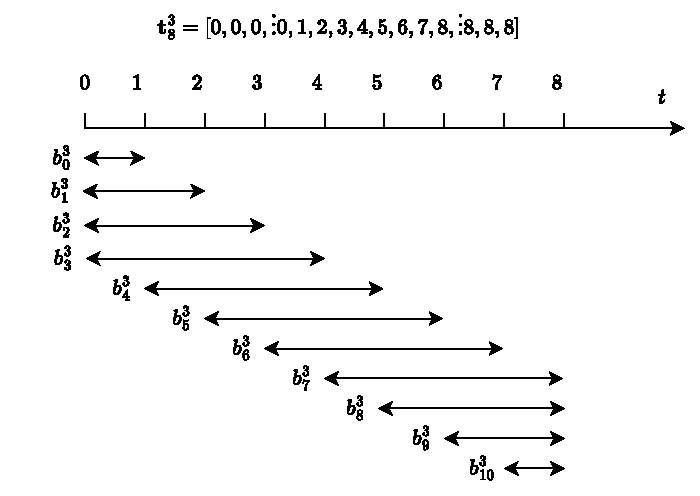
\includegraphics[width=\linewidth]{./chap5_trajectory_planning/figures/region_of_support.drawio.pdf}
  \caption{Region of support for the B-spline basis functions of degree $d=3$ with uniform clamped knot vector $\mathbf{t}_8^d$.}
  \label{fig:region_of_support}  
\end{marginfigure}

%---------------------------------------------------------------
\subsection{Convex Hull Property}

Another important property of B-splines, is that the spline $\mathbf{p}(t)$ is contained in the convex hull of its supporting control points.  In this section we formalize the convex hull property.

\begin{definition}
We say that the vector $\xbf$ is in the convex hull of the vectors $\{\mathbf{q}_1, \dots, \mathbf{q}_n\}$ if 
\[
\xbf = \sum_{j=1}^n \alpha_j \mathbf{q}_j, \qquad \text{where} \qquad \sum_{j=1}^n \alpha_j = 1.
\]	
\end{definition}

We first show that at any instant of time $t\in\text{span}(\mathbf{t}_M^b)$, the b-spline basis functions sum to unity.   

\begin{lemma} \label{lem:basis_vectors_sum_to_1}
	Let $\mathbf{t}_M^d$ be a natural knot vector.  Then for any instant of time $t\in\text{span}(\mathbf{t})$, the basis vectors at that time sum to unity.  In particular, if $t\in[t_j, t_{j+1}]\subset\text{span}(\mathbf{t})$, for $j\in[0,M-1]$, then
	\[
	\sum_{m=0}^{M+d-1} b_m^d(t, \mathbf{t}_M^d) =
	\sum_{m=j}^{j+d} b_m^d(t, \mathbf{t}_M^d) = 1.
	\]
\end{lemma}
\begin{proof}  The proof follows from Lemma~\ref{lem:nonzero_basis_vectors}, a careful, but straight-forward accounting using Equations~\eqref{eq:spline_basis_definition_0} and~\eqref{eq:spline_basis_definition_k}.	
\end{proof}


\begin{lemma}\label{lem:spline_in_convex_hull}
	Let $\mathbf{t}_M^d$ be a natural knot vector. 
	If $t\in[t_j, t_{j+1}]\subset\text{span}(\mathbf{t})$, for $j\in[0,M-1]$, then the B-spline
	\[
	\mathbf{p}(t) = \sum_{m=0}^{M+d-1} \cbf_m b_m^d(t, \mathbf{t}_M^d) = \sum_{m=j}^{j+d} \cbf_m b_m^d(t,  \mathbf{t}_M^d)
	\]
	is in the convex hull of the control points $\{\cbf_j, \dots, \cbf_{j+d}\}$.
\end{lemma}
\begin{proof}
	The lemma follows from Lemma~\ref{lem:basis_vectors_sum_to_1} and Corollary~\ref{lem:finite_num_control_points}.
\end{proof}
Lemma~\ref{lem:spline_in_convex_hull} is an important result for path planning since we can guarantee collision-free paths by simply checking that the convex hull of control points is collision free.

%---------------------------------------------------------
\par\noindent{\bf SciPy BSpline library}
The SciPy library has a B-spline library.  

The following commands will create a cubic spline.
\begin{lstlisting}
import numpy as np
from scipy.interpolate import BSpline
	
	
def uniform_clamped_knots(k, M, t0=np.inf, tf=np.inf):
    # k is the order, M is the number of time intervals
    knots = [0] * k + list(range(0, M + 1)) + [M] * k
    knots = np.asarray(knots)  # convert knots to an NP array
    if t0 != np.inf:
        if (tf != np.inf) & (tf > t0):
            knots = (tf-t0)/M * knots
        knots = knots + t0
    return knots	

t0 = 1 # initial time
tf = 5 # final time
k = 3  # spline order
M = 3  # number of time intervals
knots = uniform_clamped_knots(k=order, M=M, t0=t0, tf=tf)
# need M+k control points
ctrl_pts = np.array([[0, 0, 0],  
                     [0, 1, 0],
                     [0, 0, 1],
                     [0, 1, 1],
                     [1, 1, 0],
                     [1, 1, 1]])
spl = BSpline(t=knots, c=ctrl_pts, k=order)
plot_spline(spl)
\end{lstlisting}

Where {\tt plot\_spline} is given below.
\begin{lstlisting}
from math import ceil
from scipy.interpolate import BSpline
import matplotlib.pyplot as plt

def plot_spline(spl):
    t0 = spl.t[0]  # first knot is t0
    tf = spl.t[-1]  # last knot is tf
    # number of points in time vector so spacing is 0.01
    N = ceil((tf - t0)/0.01)
    t = np.linspace(t0, tf, N)  # time vector
    position = spl(t)
    # 3D trajectory plot
    fig = plt.figure(1)
    ax = fig.add_subplot(111, projection='3d')
    # plot control points (convert YX(-Z) -> NED)
    ax.plot(spl.c[:, 1], spl.c[:, 0], -spl.c[:, 2],
            '-o', label='control points')
    # plot spline (convert YX(-Z) -> NED)
    ax.plot(position[:, 1], position[:, 0], -position[:, 2],
            'b', label='spline')
    ax.legend()
    ax.set_xlabel('x', fontsize=16, rotation=0)
    ax.set_ylabel('y', fontsize=16, rotation=0)
    ax.set_zlabel('z', fontsize=16, rotation=0)
    #ax.set_xlim3d([-10, 10])
    plt.show()
\end{lstlisting}

The resulting spline is shown in Figure~\ref{fig:example_spline_curve}.
\begin{marginfigure}[0in]
  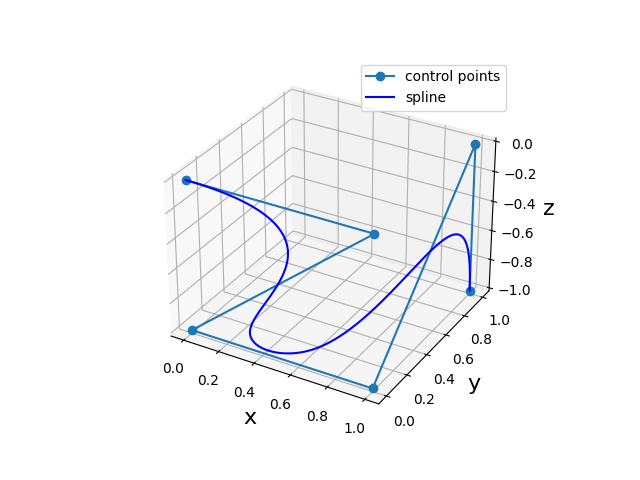
\includegraphics[width=\linewidth]{./chap5_trajectory_planning/figures/example_spline_curve}
  \caption{Example spline curve}
  \label{fig:example_spline_curve}  
\end{marginfigure}

%+++++++++++++++++++++++++++++++
\subsection{Derivatives of B-splines}


To simplify notation we will stack the basis function in a vector as
\begin{equation}\label{eq:basis_vector}
\bbf_M^d(t) \defeq \begin{pmatrix} b_0^d(t, \mathbf{t}_M^d) \\ b_1^d(t, \mathbf{t}_M^d) \\ \vdots \\ b_{M+d-1}^d(t, \mathbf{t}_M^d) \end{pmatrix}, 
\end{equation}
and the control points as a matrix 
\[
\Cbf = \begin{pmatrix} \cbf_0 & \cbf_1 & \dots & \cbf_{M+d-1} \end{pmatrix}
\]
allowing Equation~\eqref{eq:general-b-spline} to be written as
\[
\mathbf{p}(t) = \Cbf \bbf_M^d(t), \qquad t\ in\text{span}(\mathbf{t}_M^d).
\]
%1Given the shift and scale invariance of the B-spline basis functions, $\mathbf{p}(t)$ can be shifted and scaled to represent functions over arbitrary finite time intervals.

%For parameterized paths $\mathbf{p}(\sigma)$, where the path parameter $\sigma\in[0,1]$ we set the knot vector as $\frac{1}{M}\mathbf{t}_{M}^k$
%and the parameterized B-spline is given by
%\[
%\mathbf{p}(\sigma) = \Cbf \bbf_M^k(\sigma; \frac{1}{M}\mathbf{t}_{M}^k), \qquad \sigma\in[0, 1].
%\]
%Abusing notation, we will use $\bbf_M^k(\sigma)$ to mean $\bbf_M^k(\sigma; \frac{1}{M}\mathbf{t}_{M}^k)$, and parameterized paths with always be defined for $\sigma\in[0,1]$


We begin this section by noting that the basis functions and the knot vector do not have to be of the same degree.  In fact, if the knot vector has higher degree than the basis functions, then the first several basis functions will simply be zero.  
For example, let $\mathbf{t}_3^2 = [0, 0,\vdots 0, 1, 2, 3, \vdots 3, 3]$, then from Equation~\eqref{eq:spline_basis_definition_0} $b_0^0(t,  \mathbf{t}_3^2)$, $b_1^0(t,  \mathbf{t}_3^2)$, $b_5^0(t,  \mathbf{t}_3^2)$, $b_6^0(t,  \mathbf{t}_3^2)$, $b_0^1(t,  \mathbf{t}_3^2)$, and $b_5^1(t,  \mathbf{t}_3^2)$ are equal to zero since the knot intervals in the denominator for those functions are zero.  The remaining basis functions are shown in Figure~\ref{fig:shifting_property}.
\begin{marginfigure}[0in]
  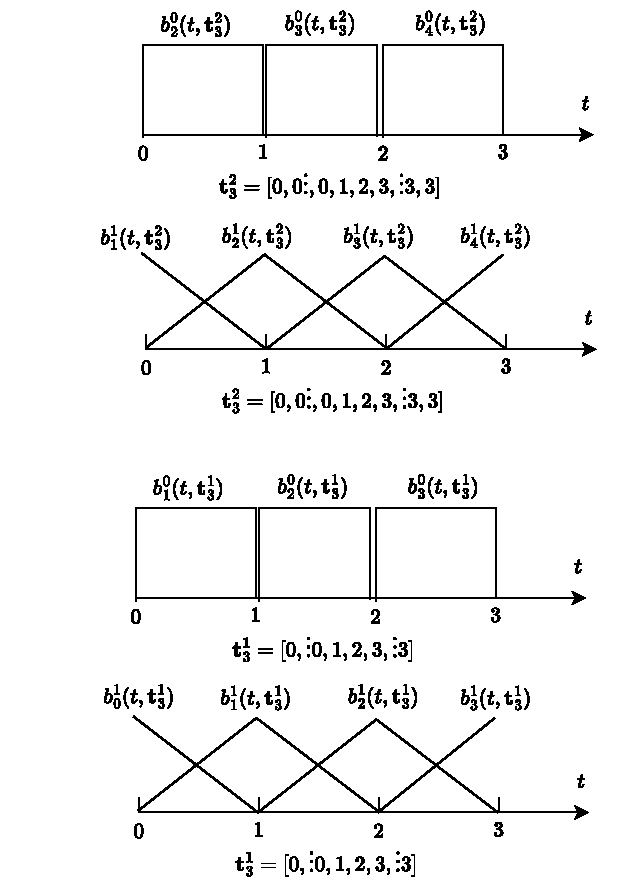
\includegraphics[width=\linewidth]{./chap5_trajectory_planning/figures/shifting_property.drawio}
  \caption{Shifting property of uniform clamped B-spline basis functions.}
  \label{fig:shifting_property}  
\end{marginfigure}
If on the other hand, the knot vector has one degree lower, i.e., $\mathbf{t}_3^1 = [0,\vdots 0, 1, 2, 3, \vdots 3]$, then the basis vectors are also shown to the right in Figure~\ref{fig:shifting_property}.  It is clear that reducing the degree of the knot vector by one, shifts the index of the basis vectors by one.  We can formalize these observations in the following lemma.
\begin{lemma} \label{lem:shifting_property}
For natural knot vectors $\mathbf{t}_M^d \in \mathbb{R}^{M+2d+1}$ and $\mathbf{t}_M^{d+1}\in\mathbb{R}^{M+2d-1}$ we have for $t\in\text{span}(\mathbf{t}_M^d)=\text{span}(\mathbf{t}_M^{d+1})$,
\[
b_m^j(t,  \mathbf{t}_M^d) = b_{m+1}^j(t,  \mathbf{t}_M^{d+1}), \qquad j \leq d, \qquad m = 0, \dots, M+1+2(d-j).
\]	
Using vector notation we have that
\[
\underbrace{\bbf_M^{j}(t,  \mathbf{t}_M^{d})}_{(M+1+2d)\times 1} = S_{M+1+2d} \underbrace{\bbf_M^{j}(t,  \mathbf{t}_M^{d+1})}_{(M+1+2(d+1))\times 1},
\]
where
\[
	S_{N} \defeq \begin{bmatrix} \mathbf{0}_{N\times 1}, & \mathbf{I}_{N\times N}, & \mathbf{0}_{N\times 1} \end{bmatrix}.
\]
\end{lemma}
\begin{proof}
Let
\begin{align*}
\mathbf{t}_M^{d+1} &= [\hat{\tau}_{0}, \hat{\tau}_{1}, \dots, \hat{\tau}_{d+1}, \dots, \hat{\tau}_{M+d+2}, \dots, \hat{\tau}_{M+2d+2}, \hat{\tau}_{M+2d+3}] \\
				   &= [t_{-d-1}, t_{-d}, \dots, t_{0}, \dots, t_M, \dots, t_{M+d}, t_{M+d+1}] \\
\mathbf{t}_M^{d}   &= [\tau_{0}, \dots, \tau_{d}, \dots, \tau_{M+d+1}, \dots, \tau_{M+2d+1}] \\f
				   &= [t_{-d}, \dots, t_{0}, \dots, t_M, \dots, t_{M+d}],
\end{align*}	
where it is clear that $\tau_j = \hat{\tau}_{j+1}$.  Therefore, from Equations~\eqref{eq:spline_basis_definition_0}we have
\begin{align*}
b_m^0(t, \mathbf{t}_M^d) &= \begin{cases} 1 & \text{~if~} \tau_m \leq t \leq \tau_{m+1} \\ 
 									 0 & \text{~otherwise} 
 					   		\end{cases} \\
 					   	 &= \begin{cases} 1 & \text{~if~} \hat{\tau}_{m+1} \leq t \leq \hat{\tau}_{m+2} \\ 
 									 0 & \text{~otherwise} 
 					   		\end{cases} \\
 					   	 &= b_{m+1}^0(t, \mathbf{t}_M^{d+1}). 
\end{align*}
Equations~\eqref{eq:spline_basis_definition_k} and~\eqref{eq:spline_basis_definition_w} follow by similar manipulation. 
\end{proof}


We have the following lemma which gives the general formula for the derivative of the spline basis.
\begin{lemma}\label{lem:derivative_basis_functions}
If $\mathbf{t}_M^d$ is a natural knot vector, then the $\ell^{th}$ derivative of the degree $d$ spline function with  $0\leq \ell \leq d+1$, is given by
\[
\frac{d^\ell}{dt^\ell}b_m^{d}(t,  \mathbf{t}_M^d) = d\left(\frac{\frac{d^{\ell-1}}{dt^{\ell-1}}b_m^{d-1}(t,  \mathbf{t}_M^d)}{\tau_{m+d}-\tau_m} - \frac{\frac{d^{\ell-1}}{dt^{\ell-1}}b_{m+1}^{d-1}(t,  \mathbf{t}_M^d)}{\tau_{m+d+1}-\tau_{m+1}} \right).
\]	
\end{lemma}
\marginnote{
The proof of Lemma~\ref{lem:derivative_basis_functions} is in~\cite{PieglTiller95}.
}

Using vector notation, we have the following formula for the derivative of a spline function.
\begin{lemma} \label{lem:derivative_of_spline}
Given the natural spline function of degree $d$
\[
\mathbf{p}(t) = \Cbf \bbf_M^d(t), \quad t\in\text{span}(\mathbf{t}_M^d)
\]
we have that
\[
\frac{d\mathbf{p}}{dt}(t) = \Cbf D_M^d \bbf_M^{d-1}(t), \quad t\in\text{span}(\mathbf{t}_M^{d-1})
\]	
where $D_M^d$ is the $(M+d)\times (M+d-1)$ derivative matrix given by
\begin{equation}\label{eq:D_d}
D_M^d = -\begin{bmatrix}\bar{D}_M^d \\ \mathbf{0}_{1\times(M+d-1)} \end{bmatrix} + \begin{bmatrix}\mathbf{0}_{1\times(M+d-1)} \\ \bar{D}_M^d \end{bmatrix},
\end{equation}
where
\begin{equation}\label{eq:D_d_bar}
\bar{D}_M^d = \text{diag}\left(\frac{d}{t_{-d+1}-t_1}, \frac{d}{t_{-d+2}-t_2}, \dots,  \frac{d}{t_{M+2d-2}-t_{M+d-2}}\right),
\end{equation}
is an $(M+d-1)\times(M+d-2)$ diagonal matrix.
\end{lemma}
\begin{proof}
Let
\begin{align*}
\mathbf{t}_M^{d} &= [\hat{\tau}_{0}, \hat{\tau}_{1}, \dots, \hat{\tau}_{d}, \dots, \hat{\tau}_{M+d}, \dots, \hat{\tau}_{M+2d-1}, \hat{\tau}_{M+2d}] \\
				   &= [t_{-d}, t_{-d+1} \dots, t_{0}, \dots, t_M, \dots, t_{M+d-1}, t_{M+d}] \\
\mathbf{t}_M^{d-1}   &= [\tau_{0}, \dots, \tau_{d-1}, \dots, \tau_{M+d-1}, \dots, \tau_{M+2d-2}] \\
				   &= [t_{-d+1}, \dots, t_{0}, \dots, t_M, \dots, t_{M+d-1}],
\end{align*}	
where it is clear that $\tau_j = \hat{\tau}_{j+1}$, for $j=0,\dots,M+2d-2$.

Noting that
\[
\mathbf{p}(t) = \Cbf \bbf_M^d(t)
              = \sum_{m=0}^{M+d-1} \cbf_m b_m^d(t,  \mathbf{t}_M^d),
\]
we have that
\[
\frac{d\mathbf{p}}{dt} = \sum_{m=0}^{M+d-1} \cbf_m \frac{d b_m^d(t,  \mathbf{t}_M^d)}{dt}.
\]
From Lemma~\ref{lem:derivative_basis_functions} we get
\begin{align*}
\frac{d\mathbf{p}}{dt} &= \sum_{m=0}^{M+d-1}  \cbf_m (d) \left(\frac{b_m^{d-1}(t,  \mathbf{t}_M^d)}{\hat\tau_{m+d}-\hat\tau_m} - \frac{b_{m+1}^{d-1}(t,  \mathbf{t}_M^d)}{\hat\tau_{m+d+1}-\hat\tau_{m+1}} \right) \\
&= \sum_{m=0}^{M+d-1} \cbf_m \left[ \left(\frac{d}{\hat\tau_{m+d}-\hat\tau_m}\right) b_m^{d-1}(t,  \mathbf{t}_M^d) - \left(\frac{d}{\hat\tau_{m+d+1}-\hat\tau_{m+1}}\right)  b_{m+1}^{d-1}(t,  \mathbf{t}_M^d) \right] \\
&= \left(\frac{d}{\hat\tau_{d}-\hat\tau_0}\right)\cbf_0 b_0^{d-1}(t,  \mathbf{t}_M^d) + \sum_{m=1}^{M+d-1} \left(\frac{d}{\hat\tau_{m+d}-\hat\tau_m}\right) \left(  \cbf_m - \cbf_{m-1}  \right) b_m^{d-1}(t,  \mathbf{t}_M^d) \\
&\qquad - \left(\frac{d}{\hat\tau_{M+2d}-\hat\tau_{M+d}}\right)\cbf_{M+d-1}b_{M+d}^{d-1}(t, \mathbf{t}_M^d).
\end{align*}
From Lemma~\ref{lem:span_of_basis_vectors} we have that $b_0^{d-1}(t, \mathbf{b}_M^d)$ and $b_{M+d}^{d-1}(t, \mathbf{b}_M^d)$ are zero on $\text{span}(\mathbf{t}_M^d)$, which implies that 
\begin{align*}
	\frac{d\mathbf{p}}{dt} 
		&= \sum_{m=1}^{M+d-1} \left(\frac{d}{\hat\tau_{m+d}-\hat\tau_m}\right) \left(  \cbf_m - \cbf_{m-1}  \right) b_m^{d-1}(t,  \mathbf{t}_M^d) \\
		&= \sum_{m=0}^{M+d-2} \left(\frac{d}{\hat\tau_{m+1+d}-\hat\tau_{m+1}}\right) \left(  \cbf_{m+1} - \cbf_{m}  \right) b_{m+1}^{d-1}(t,  \mathbf{t}_M^d) \\
		&= \sum_{m=0}^{M+d-2} \left(\frac{d}{\tau_{m+d}-\tau_{m}}\right) \left(  \cbf_{m+1} - \cbf_{m}  \right) b_{m}^{d-1}(t,  \mathbf{t}_M^{d-1}) \\	
		&= \Cbf D_M^d \bbf_M^{d-1}(t).	
\end{align*}
\end{proof}

Note that if $\mathbf{t}_M^d$ is the uniform knot vector in Equation~\eqref{eq:knot_vector_uniform}, then 
\[
\bar{D}_M^d  = I_{M+d-2},
\]
since the interval in the denominator is always equal to $d$.
%
Similarly, if $\mathbf{t}_M^d$ is the uniform clamped knot vector in Equation~\eqref{eq:knot_vector_uniform_clamped}, then 
\[
\bar{D}_M^d = \text{diag}\left(\frac{d}{1}, \frac{d}{2}, \dots, \frac{d}{d-1}, \underbrace{1, \dots, 1}_{M-d}, \frac{d}{d-1}, \dots, \frac{d}{2}, \frac{d}{1}\right).
\]

%
%\begin{lemma} \label{lem:derivative_of_spline_not_clamped}
%Given the $k^{th}$-order uniform spline function
%\[
%\mathbf{p}(t) = \Cbf \bbf_M^k(t), \quad t\in[0, M]
%\]
%we have that
%\[
%\frac{d\mathbf{p}}{dt}(t) = \Cbf D_M^k \bbf_M^{k-1}(t), \quad t\in[0, M]
%\]	
%where $D_M^k$ is the $(M+k-1)\times (M+k-2)$ derivative matrix given by
%\begin{equation}\label{eq:D_k}
%D_M^k = \begin{pmatrix} -1 & 0 & 0 & \dots & 0 & 0 \\ 
% 						 1 & -1 & 0 & \dots & 0 & 0 \\
% 						 0 & 1 & -1 & \dots & 0 & 0\\
% 						 \vdots & & & & & \vdots \\
% 						 0 & 0 & 0 & \vdots & 1 & -1 \\
% 						 0 & 0 & 0 & \vdots & 0 & 1
% 		\end{pmatrix}.
%\end{equation}
%\end{lemma}

%
From Lemma~\ref{lem:derivative_of_spline} we can derive a number of useful results, which we summarize in the corollary below.
\begin{corollary} \label{cor:derivatives}
	Given the natural/uniform/clamped B-spline function of degree $d$,
	\[
	\mathbf{p}(t) = \Cbf \bbf_M^d(t), \quad t\in\text{span}(\mathbf{t}_M^d)
	\]
	we can make the following statements:
	\begin{description}
	\item[(i)] The derivative  $\frac{d\mathbf{p}}{dt}$ is a natural/uniform/clamped clamped B-spline function of degree $d-1$.
	\item[(ii)] The control points of $\frac{d\mathbf{p}}{dt}$ are given by
		\[
		C^{'} \defeq C D_M^d = \begin{pmatrix}
				\frac{d}{t_{-d+1}-t_1} (\cbf_1 - \cbf_0)^\top \\
				\vdots \\
				\frac{d}{t_{M+2d-2}-t_{M_d-2}} (\cbf_{M+d-1} - \cbf_{M+d-2})^\top
 				\end{pmatrix}^\top
 			\defeq \begin{pmatrix}
 			        \cbf_0^{'\top} \\
 			        \vdots \\
 			        \cbf_{M+d-2}^{'\top}
 				   \end{pmatrix}^\top.
		\]
	\item[(iii)] The $\ell^{th}$ derivative of $\mathbf{p}(t)$ for $0\leq\ell\leq d-1$ is given by
		\begin{align*}
			\frac{d^{\ell}\mathbf{p}}{dt^{\ell}} 
			&= C D_M^d D_M^{d-1} \dots D_M^{d-\ell} \bbf_M^{d-\ell}(t), \quad t\in \text{span}(\mathbf{t}_M^d) \\
			&= C^{(\ell)} \bbf_M^{d-\ell}(t), \quad t\in \text{span}(\mathbf{t}_M^d) \\
			&= C \boldsymbol{\psi}^{(\ell)}(t), \quad t\in \text{span}(\mathbf{t}_M^d) \\
		\end{align*}
		where the control points of the $(d-\ell)^{th}$ degree spline are given by
		\[
			C^{(\ell)} = C D_M^d D_M^{d-1} \dots D_M^{d-\ell-1}
		\]
		or alternatively, the $\ell^{th}$ derivative of the basis vector $\bbf_M^d(t)$ is given by
		\[
			\boldsymbol{\psi}^{(\ell)} \defeq \frac{d^{\ell}\bbf_M^d(t)}{dt^{\ell}} = D_M^d D_M^{d-1} \dots D_M^{d-\ell} \bbf_M^{d-\ell}(t), \quad t\in \text{span}(\mathbf{t}_M^d).
		\]
	\end{description}
\end{corollary}


For uniform clamped B-splines, we have the following.

\begin{corollary} \label{cor:derivatives_clamped_splines}
	Given the uniform clamped B-spline function of degree $d$
	\[
	\mathbf{p}(t) = \Cbf \bbf_M^d(t), \quad t\in[0, M]
	\]
	we can make the following statements:
	\begin{description}
	\item[(i)] The control points of $\frac{d\mathbf{p}}{dt}$ are given by
		\[
		C^{'} \defeq C D_M^k = \begin{pmatrix}
				\frac{d}{1} (\cbf_1 - \cbf_0)^\top \\
				\vdots \\
				\frac{d}{d-1} (\cbf_{d-2} - \cbf_{d-3})^\top \\
				(\cbf_{d-1} - \cbf_{d-2})^\top \\
				\vdots \\
				(\cbf_{M+1} - \cbf_{M})^\top \\
				\frac{d}{d-1} (\cbf_{M+2}-\cbf_{M+1})^\top \\
				\vdots \\
				\frac{d}{1} (\cbf_{M+d-1} - \cbf_{M+d-2})^\top
 				\end{pmatrix}^\top
 			\defeq \begin{pmatrix}
 			        \cbf_0^{'\top} \\
 			        \vdots \\
 			        \cbf_{M+d-2}^{'\top}
 				   \end{pmatrix}^\top.
		\]
	\item[(ii)] The derivative of $\mathbf{p}(t)$ at $t=0$ is given by the difference of the first two control points as
		\[
			\frac{d\mathbf{p}}{dt}(0) = (d)(\cbf_1 - \cbf_0).
		\]
	\item[(iii)] The derivative of $\mathbf{p}(t)$ at $t=M$ is given by the difference of the last two control points as
		\[
			\frac{d\mathbf{p}}{dt}(M) = (d)(\cbf_{M+d-1} - \cbf_{M+d-2}).
		\]
	\item[(iv)] If the desired B-spline trajectory with $d\geq 3$ has the following desired endpoint conditions:
		\begin{align*}
			\text{Initial position:} &\quad \mathbf{p}(0) \stackrel{des}{=} \mathbf{p}_0 \\	
			\text{Final position:} &\quad \mathbf{p}(M) \stackrel{des}{=} \mathbf{p}_f \\
			\text{Initial velocity:} &\quad \frac{d\mathbf{p}}{dt}(0) \stackrel{des}{=} \mathbf{v}_0 \\	
			\text{Final velocity:} &\quad \frac{d\mathbf{p}}{dt}(M) \stackrel{des}{=} \mathbf{v}_f, \\
			\text{Initial acceleration:} &\quad \frac{d^2\mathbf{p}}{dt^2}(0) \stackrel{des}{=} \mathbf{a}_0 \\	
			\text{Final acceleration:} &\quad \frac{d^2\mathbf{p}}{dt^2}(M) \stackrel{des}{=} \mathbf{a}_f,
		\end{align*}
		then the first and last three control points satisfy
		\begin{align*}
			\cbf_0 &= \mathbf{p}_0 \\
			\cbf_1 &= \mathbf{p}_0 + \frac{1}{d} \mathbf{v}_0 \\
			\cbf_2 &= \mathbf{p}_0 + \frac{3}{d} \mathbf{v}_0 + \frac{2}{(d)(d-1)}\mathbf{a}_0 \\
			\cbf_{M+d-3} &= \mathbf{p}_f - \frac{3}{d}\mathbf{v}_f + \frac{2}{(d)(d-1)}\mathbf{a}_f \\
			\cbf_{M+d-2} &= \mathbf{p}_f - \frac{1}{d}\mathbf{v}_f \\
			\cbf_{M+d-1} &= \mathbf{p}_f.
		\end{align*}
	\end{description}
\end{corollary}



%---------------------------------------------------------------
\subsection{B-Spline Planning for Chains of Integrators}

%---------------------------------------------------------------
\subsection{B-Splines on Lie Groups}

%---------------------------------------------------------------
\subsection{B-Splines Surfaces}

Suppose that the objective is to create a one dimensional surface over a two dimensional domain.  For example, a terrain map is a one dimensional surface of altitudes over the north-east plane.  In this section we will explore the use of B-splines to accomplish this objective. Many of the ideas and notation in this section come from~\cite{RodriguesTsiogkasAguiar20}.

If $\mathbf{t}_M^k$ and $\mathbf{t}_N^k$ are two different $k^{th}$ order uniform knot vectors of length $M$ and $N$ understood to define knots in the $x$ and $y$ directions, then following Equation~\eqref{eq:clamped_uniform_spline}, a clamped uniform B-spline surface is defined as 
\begin{equation}\label{eq:spline_surface1}
S(x, y) \defeq \sum_{m=0}^{M+k-2} \sum_{n=0}^{N+k-2} c_{m,n} b^k_m(x; \mathbf{t}_M^k) b^k_n(y; \mathbf{t}_N^k), \quad x\in[0,M], y\in[0, N],
\end{equation}
where $c_{m, n}$, $m=0, \dots, M+k-2$, $n=0, \dots, N+k-2$ are the control points of the surface.  Defining the matrix $\Cbf=\{c_{m,n}\}$, and defining the spatial variable $\sbf = (s_1, s_2)^\top$, we can write Equation~\eqref{eq:spline_surface1} as
\begin{equation}\label{eq:spline_surface2}
S(\sbf) = \bbf^k_M(s_1)^\top \Cbf \bbf^k_N(s_2), \quad \sbf\in[0, M]\times[0, N],
\end{equation}
This equation is linear in the spline coefficients $\Cbf$.  In other words, if $S_1(\sbf)=\bbf^k_M(s_1)^\top \Cbf_1 \bbf^k_N(s_2)$, and $S_1(\sbf)=\bbf^k_M(s_1)^\top \Cbf_2 \bbf^k_N(s_2)$ are two different spline surfaces, then 
\[
S(\sbf)\defeq \alpha S_1(\sbf) + \beta S_2(\sbf) = \bbf^k_M(s_1)^\top \left(\alpha\Cbf_1 + \beta\Cbf_2\right) \bbf^k_N(s_2),
\]
is also a spline surface.

Suppose that instead of defining the surface over the set $[0, M]\times[0, N]$ we instead would like to define the surface over the set $[\underline{X}, \overline{X}]\times[\underline{Y}, \overline{Y}]$.  Given the shift and scaling properties is Lemmas~\ref{lem:basis_are_shift_invariant} and~\ref{lem:bases_are_scale_invariant} we have 
\begin{equation}\label{eq:spline_surface3}
S(\sbf) = \bbf^k_M\left(\frac{M(s_1-\underline{X})}{\overline{X}-\underline{X}}\right)^\top \Cbf \bbf^k_N\left(\frac{N(s_2-\underline{Y})}{\overline{Y}-\underline{Y}}\right), \quad \sbf\in[\underline{X}, \overline{X}]\times[\underline{Y}, \overline{Y}].
\end{equation}

\begin{marginfigure}[0in]
  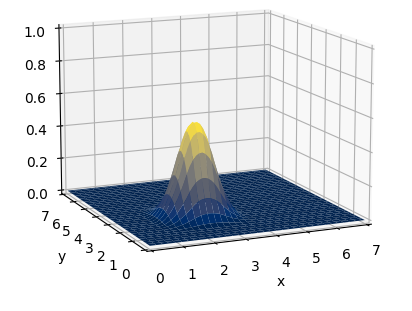
\includegraphics[width=\linewidth]{./chap5_trajectory_planning/figures/spline_surface_basis}
  \caption{A single second order spline bases function $b_3^2(s_1)b_3^2(s_2)$.}
  \label{fig:spline_surface_bases}  
\end{marginfigure}


%
%The basic idea is to create two-dimensional bases vectors as the tensor product of the one-dimensional bases vectors introduced in Section~\ref{sec:b-spline-basis-functions}.  For example, replacing the time variable $t$ with the spacial variables $x$ and $y$, the $k^{th}$-order two dimensional basis vectors are defined as
%\[
%b^k_{m,n}(x,y) = b^k_m(x; \mathbf{t}_1) b^k_n(y; \mathbf{t}_2), 
%\]
%where $T=\mathbf{t}_1 \times \mathbf{t}_2$ is the two-dimensional knot array, and $b^{k}_m(x; \mathbf{t}_1)$ is the $k^{th}$-order spline function with index $m$ and knot vector $\mathbf{t}_1$, and similarly for $b^k_n(y; \mathbf{t}_2)$.
%
%
%If $\mathbf{t}_M^k$ and $\sbf_N^k$ are $k^{th}$ order uniform clamped knot vectors of length $M$ and $N$, then 
%$\mathbf{T}^k_{M,N}\defeq \mathbf{t}_M^k \times \sbf_M^k$ is a $k^{th}$ order uniform clamped knot array of size (M,N).  For example, if $\mathbf{t}_3^2 = [0, 0, 0, 1, 2, 3, 3, 3]$, and $\sbf_2^2 = [0, 0, 0, 1, 2, 2, 2]$, then
%\[
%\mathbf{T}^2_{3,2} = \begin{bmatrix} 
%						(0, 0) & (0, 0) & (0, 0) & (0, 1) & (0, 2) & (0, 2) & (0, 2) \\
%						(0, 0) & (0, 0) & (0, 0) & (0, 1) & (0, 2) & (0, 2) & (0, 2) \\
%						(0, 0) & (0, 0) & (0, 0) & (0, 1) & (0, 2) & (0, 2) & (0, 2) \\
%						(1, 0) & (1, 0) & (1, 0) & (1, 1) & (1, 2) & (1, 2) & (1, 2) \\
%						(2, 0) & (2, 0) & (2, 0) & (2, 1) & (2, 2) & (2, 2) & (2, 2) \\
%						(3, 0) & (3, 0) & (3, 0) & (3, 1) & (2, 2) & (3, 2) & (3, 2) \\
%						(3, 0) & (3, 0) & (3, 0) & (3, 1) & (2, 2) & (3, 2) & (3, 2) \\
%						(3, 0) & (3, 0) & (3, 0) & (3, 1) & (2, 2) & (3, 2) & (3, 2)
% 					 \end{bmatrix}.
%\]
%
%
%Recall that if $\mathbf{A}$ is an $m\times n$ matrix and $\bbf$ is $p\times q$ matrix, then the Kronecker product of $\mathbf{A}$ and $\bbf$ is defined as 
%\[
%\mathbf{A}\otimes\bbf \circeq \begin{pmatrix} 
% 										a_{11}B & a_{12}B & \dots & a_{1n}B \\	
% 										a_{21}B & a_{22}B & \dots & a_{2n}B \\
% 										\vdots & \vdots & \dots & \vdots \\
% 										a_{m1}B & a_{m2}B & \dots & a_{mn}B \\	
% 									\end{pmatrix}.
%\]
%We will use the Kronecker product to simplify the notation associated with spline surfaces.  Let $\xbf=(x_1, x_2)^\top\in\mathbb{R}^2$, and let $\bbf^k_M(x_1; \mathbf{t}_M^k)$ and $\bbf^k_N(x_2; \sbf_N^k$ be $k^{th}$ order basis vectors as defined in Equation~\eqref{eq:basis_vector} and $T^k_{M,N}=\mathbf{t}_M^k \times \sbf_N^k$, then define the basis vector 
%\[
%\bbf^k_{M,N}(\xbf; T^k_{M,N}) = \bbf^k_M(x_1; \mathbf{t}_M^k) \otimes \bbf^k_N(x_2; \sbf_N^k), 
%\]
%where we will drop to inclusion of the knot array and write simply $\bbf^k_{M,N}(\xbf)\circeq\bbf^k_{M,N}(\xbf; T^k_{M,N})$.
%Similarly, defining the control vector 
%\[
%\cbf \circeq \begin{pmatrix} c_{1,1} & c_{1,2} & \dots & c_{1,N} & \dots & c{M,1} & \dots & c_{M,N} \end{pmatrix}^\top,
%\]
%we get that
%\[
%S^k(\xbf) = \cbf^\top  \bbf^k_{M,N}(\xbf), \qquad \xbf \in [0,M]\times[0,N].
%\]

The Python code below plots a randomly defined terrain map over the domain $[-\pi, \pi]\times[-2\pi, 2\pi]$.
\begin{lstlisting}
import numpy as np
import splipy as sp
import matplotlib.pyplot as plt
from bspline_tools import uniform_clamped_knots

def draw_random_surface(order=2, M=10, N=10,
                        Xmin=-3.14159, Xmax=3.14159,
                        Ymin=-2*3.14159, Ymax=2*3.14159):
    # define the spline surface
    knots_x = uniform_clamped_knots(k=order, M=M)
    knots_y = uniform_clamped_knots(k=order, M=N)
    basis_x = sp.BSplineBasis(order + 1, knots_x)
    basis_y = sp.BSplineBasis(order + 1, knots_y)
    C = np.random.rand(M + order, N + order)  # random control points
    surface = sp.Surface(basis_x, basis_y,
                         np.reshape(C, ((M + order) * (N + order), 1)))
    # plot the spline surface
    x = np.linspace(Xmin, Xmax, 10 * M)
    y = np.linspace(Ymin, Ymax, 10 * N)
    S = surface(M*(x-Xmin)/(Xmax-Xmin),
                N*(y-Ymin)/(Ymax-Ymin))  # surface points
    fig = plt.figure()
    ax = fig.add_subplot(111, projection='3d')
    plt.xlabel('x')
    plt.ylabel('y')
    x_pts, y_pts = np.meshgrid(x, y)  # grid points
    ax.plot_surface(x_pts, y_pts, S[:, :, 0])
    plt.show()
\end{lstlisting}
The result of running this code is shown in Figure~\ref{fig:random_spline_surface}
\begin{marginfigure}[0in]
  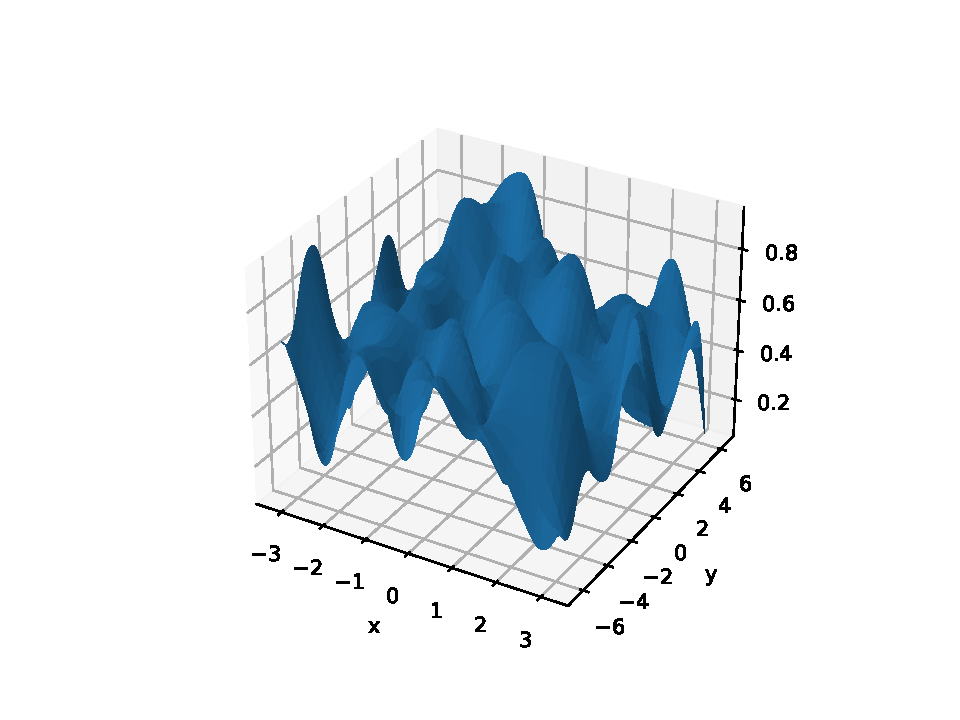
\includegraphics[width=\linewidth]{./chap5_trajectory_planning/figures/random_spline_surface}
  \caption{Spline surface with randomly generated control points.}
  \label{fig:random_spline_surface}  
\end{marginfigure}




%----------------------------------
\section{Minimum Snap Trajectories}

Because multirotor dynamics are differentially flat, their motion can be completely parametrized by trajectories in position and heading.  It is argued in (Mellinger \& Kumar, 2011)~\cite{MellingerKumar11} that since acceleration is dependent on third derivative of position, and torque is dependent on the derivative of heading, that smooth trajectories for quadrotors should minimize the fourth derivative (snap) of the position spline, and the second derivative of the yaw spline.  In this section, will show to derive quadratic cost functions on the spline coefficients that minimize the appropriate derivative.  

Let the position and heading trajectories be defined by $k^{th}$ order splines over the time interval $t\in[0,M]$ as
\begin{align*}
	\mathbf{p}_d(t) &= \mathbf{C}_p b_M^k(t) \\	
	\psi_d(t) &= \mathbf{C}_{\psi} b_M^k(t),
\end{align*}
where $\mathbf{C}_p \in \mathbb{R}^{3\times M+k-1}$, and $\mathbf{C}_{\psi} \in \mathbb{R}^{1\times M+k-1}$.
As shown in Lemma~\ref{cor:derivatives_clamped_splines}, the fourth derivative of position and second derivative of heading are given by
\begin{align*}
	\mathbf{p}^{(4)}_d(t) &= \mathbf{C}_p D_M^k D_M^{k-1} D_M^{k-2} D_M^{k-3}	\mathbf{b}_M^{k-4}(t) \\
	\psi^{(2)}_d(t) &= \mathbf{C}_{\psi} D_M^k D_M^{k-1} \mathbf{b}_M^{k-2}(t).
\end{align*}
Defining
\[
S_M^{k,j} \defeq D_M^k D_M^{k-1}\cdots D_M^{k-j}
\]
gives
\begin{align*}
	\mathbf{p}^{(4)}_d(t) &= \mathbf{C}_p S_M^{k,3} 	\mathbf{b}_M^{k-4}(t) \\
	\psi^{(2)}_d(t) &= \mathbf{C}_{\psi} S_M^{k,1} \mathbf{b}_M^{k-2}(t).
\end{align*}

The normed integral square of the fourth derivative of $\mathbf{p}(t)$ is given by
\begin{align*}
	\int_0^M \norm{\mathbf{p}^{(4)}(t)}^2 \, dt
		&= 	\int_0^M \mathbf{p}^{(4)\top}(t)\mathbf{p}^{(4)}(t) \, dt \\
		&= 	\int_0^M 	{\mathbf{b}_M^{k-4}(t)}^\top {S_M^{k,3}}^\top 
				\mathbf{C}_p^\top \mathbf{C}_p S_M^{k,3} 	\mathbf{b}_M^{k-4}(t) \, dt \\
		&= 	\trace{\int_0^M 	{\mathbf{b}_M^{k-4}(t)}^\top {S_M^{k,3}}^\top 
				\mathbf{C}_p^\top \mathbf{C}_p S_M^{k,3} 	\mathbf{b}_M^{k-4}(t) \, dt } \\
		&= 	\trace{\int_0^M 	\mathbf{C}_p S_M^{k,3} 	\mathbf{b}_M^{k-4}(t) {\mathbf{b}_M^{k-4}(t)}^\top {S_M^{k,3}}^\top 
				\mathbf{C}_p^\top  \, dt } \\
		&= 	\trace{ \mathbf{C}_p S_M^{k,3} \int_0^M 	\mathbf{b}_M^{k-4}(t) {\mathbf{b}_M^{k-4}(t)}^\top \, dt~~ {S_M^{k,3}}^\top 
				\mathbf{C}_p^\top }.
\end{align*}
Define
\[
W_M^{k,j} \defeq S_M^{k,j} \int_0^M 	\mathbf{b}_M^{k-j}(t) {\mathbf{b}_M^{k-j}(t)}^\top \, dt~~ {S_M^{k,j}}^\top,
\]
and note that $W_M^{k,j}$ are constant matrices that can be pre-computed and stored in memory,
then 
\begin{align*}
\int_0^M \norm{\mathbf{p}^{(4)}(t)}^2 \, dt &= \trace{\mathbf{C}_p W_M^{k,4} \mathbf{C}_p^\top } \\
\int_0^M \abs{\psi^{(2)}(t)}^2 \, dt &= \trace{\mathbf{C}_\psi W_M^{k,1} \mathbf{C}_\psi^\top }.
\end{align*}

The initial and final conditions place constraints on the control points as shown in Corollary~\ref{cor:derivatives_clamped_splines}.  These conditions can be stated as matrix equality constraints on the control points.  For example, for fourth order splines, where the initial and final position, velocity, and acceleration are specified, we have from Corollary~\ref{cor:derivatives_clamped_splines} that
\begin{align*}
			\cbf_0 &= \mathbf{p}_0 \\
			\cbf_1 &= \mathbf{p}_0 + \frac{1}{k-1} \mathbf{v}_0 \\
			\cbf_2 &= \mathbf{p}_0 + \frac{3}{k-1} \mathbf{v}_0 + \frac{2}{(k-1)(k-2)}\mathbf{a}_0 \\
			\cbf_{M+k-4} &= \mathbf{p}_f - \frac{3}{k-1}\mathbf{v}_f + \frac{2}{(k-1)(k-2)}\mathbf{a}_f \\
			\cbf_{M+k-3} &= \mathbf{p}_f - \frac{1}{k-1}\mathbf{v}_f \\
			\cbf_{M+k-2} &= \mathbf{p}_f.
\end{align*}
which can be written in matrix form as
\begin{multline*}
	\underbrace{\begin{pmatrix}\mathbf{c}_0 & \dots \mathbf{c}_{M+k-2} \end{pmatrix}}_{\mathbf{C}_p}
	\underbrace{\begin{pmatrix} \mathbf{e}_1 & \mathbf{e}_2 & \mathbf{e}_3 & \mathbf{e}_{M+k-3} & \mathbf{e}_{M+k-2} & \mathbf{e}_{M+k-1} \end{pmatrix}}_{U_1}
	\\ = 
	\underbrace{\begin{pmatrix}\mathbf{p}_0 & \mathbf{v}_0 & \mathbf{a}_0 & \mathbf{a}_f & \mathbf{v}_f & \mathbf{p}_f \end{pmatrix}}_{A_p}
	\underbrace{\begin{pmatrix} 1 & 1 & 1 & 0 & 0 & 0 \\ 0 & \frac{1}{k-1} & \frac{3}{k-1} & 0 & 0 & 0 \\ 0 & 0 & \frac{2}{(k-1)(k-2)} & 0 & 0 & 0 \\ 0 & 0 & 0 & \frac{2}{(k-1)(k-2)} & 0 & 0 \\ 0 & 0 & 0 & \frac{-3}{k-1} & \frac{-1}{k-1} & 0 \\ 0 & 0 & 0 & 1 & 1 & 1 \end{pmatrix}}_{B^{k,4}}.
\end{multline*}


The minimum-snap problem without obstacles, can therefore be written as
\begin{equation}
	\label{eq:min_snap_no_obstacles}
	\begin{aligned}
	&\min_{\mathbf{C}_p} \trace{\mathbf{C}_p W_M^{k,4} \mathbf{C}_p^\top} \\
	&\text{subject to } \: \mathbf{C}_p U_1 = A_p B^{k,4}. 
	\end{aligned}
\end{equation}

%---------------------------------------------------
\subsection{Minimum snap trajectories without obstacles}

Without obstacles, the minimum-snap problem has an analytic solution as derived in the next theorem.
\begin{theorem}
	The optimization problem given in Equation~\eqref{eq:min_snap_no_obstacles} has an analytic solution given by
	\begin{equation}
		\mathbf{C}_p^\star  = A_p B^{k,4} U_1^\top \left(I-W_M^{k,4}U_2(U_2^\top W_M^{k,4} U_2)^{-1}U_2^\top\right),
	\end{equation}
	where
	\[
	U_2 = \begin{pmatrix} \mathbf{e}_4, \dots, \mathbf{e}_{M+k-4} \end{pmatrix}.
	\]
\end{theorem}
\proof
	We begin by noting that $U_1^\top U_1=I_{6\times 6}$ and that $U_2^\top U_1 = 0$.  Let $\check{\mathbf{C}}_p= A_pB^{k,4} U_1^\top + Z U_2^\top$ and note that
	\begin{align*}
		\check{\mathbf{C}}_pU_1 
			&= \left(	A_p B^{k,4} U_1^\top + Z U_2^\top \right) U_1 \\
			&= A_p B^{k,4} U_1^\top U_1 + Z U_2^\top U_1  \\
			&= A_p B^{k,4}.
	\end{align*}
	Therefore $\check{\mathbf{C}}_p$ satisfies the inequality constraints and implies that the optimal solution has the form of 
	\[
		\mathbf{C}_p^\ast = A_p B^{k,4} U_1^\top + Z^\ast U_2^\top.
	\]
	We have therefore transformed the constrained optimization problem in~\ref{eq:min_snap_no_obstacles} to the unconstrained optimization problem
	\begin{align*}
	&\min_{Z} \trace{\left(A_pB^{k,4} U_1^\top + Z U_2^\top\right) W_M^{k,4} \left(A_pB^{k,4} U_1^\top + Z U_2^\top\right)^\top} \\
	= &\min_{Z} \trace{A_pB^{k,4} U_1^\top W_M^{k,4} U_1 B^{k,4\top} A_p^\top + Z U_2^\top W_M^{k,4} U_1 B^{k,4\top}A_p^\top +  A_p B^{k,4} U_1\top W_M^{k,4} U_2 Z^\top + Z U_2^\top W_M^{k,4} U_2 Z^\top} \\
	= &\min_{Z} \trace{A_p B^{k,4} U_1^\top W_M^{k,4} U_1 B^{k,4\top}A_p^\top + 2Z U_2^\top W_M^{k,4} U_1 B^{k,4\top}A_p^\top + Z U_2^\top W_M^{k,4} U_2 Z^\top},
	\end{align*}
	where we have used the fact that $\trace{M^\top}=\trace{M}$.
	Letting
	\[
		J = \trace{A_p B^{k,4} U_1^\top W_M^{k,4} U_1 B^{k,4\top}A_p^\top + 2Z U_2^\top W_M^{k,4} U_1 B^{k,4\top}A_p^\top + Z U_2^\top W_M^{k,4} U_2 Z^\top}
	\]
	and recalling that for matrix equations
	\begin{align*}
		\frac{\partial}{\partial X}\trace{XM} &= M^\top \\	
		\frac{\partial}{\partial X}\trace{XMX^\top} &= X(M+M^\top),
	\end{align*}
	we get that
	\[
	\frac{\partial J}{\partial Z} = 2 A_pB^{k,4} U_1^\top W_M^{k,4} U_2 + 2 Z U_2^\top W_M^{k,4} U_2, 
	\]
	where we have used the fact that $W_M^{k,j}$ is symmetric.  Setting $\frac{\partial J}{\partial Z}$ to zero and solving for the optimal $Z$ gives
	\[
	Z^\ast = -A_p B^{k,4} U_1^\top W_M^{k,4} U_2 (U_2^\top W_M^{k,4} U_2)^{-1}.
	\]
	Therefore
	\begin{align*}
		\mathbf{C}_p^\ast 
			&= A_p B^{k,4} U_1^\top + Z^\ast U_2^\top \\	
			&= A_p B^{k,4} U_1^\top + \left(-A_p B^{k,4} U_1^\top W_M^{k,4} U_2 (U_2^\top W_M^{k,4} U_2)^{-1}\right) U_2^\top \\	
			&= A_p B^{k,4} U_1^\top \left( I - W_M^{k,4} U_2 (U_2^\top W_M^{k,4} U_2)^{-1} U_2^\top \right).	
	\end{align*}
\endproof
This is a very nice result in the sense that the matrix
\[
Q_M^{k,4} = B^{k,4} U_1^\top \left(I-W_M^{k,4}U_2(U_2^\top W_M^{k,4} U_2)^{-1}U_2^\top\right)
\]
is a constant, problem independent matrix that can be pre-computed and stored in memory, and the optimal control points can be computed simply from the initial and final conditions as 
\[
\mathbf{C}_p^\ast = A_p Q_M^{k,4}.
\]

For the heading spline, we assume constraints on the initial and final heading as
\begin{align*}
	\psi_0 &= \psi_d(0) = \mathbf{C}_\psi b_M^k(0) = c_{\psi,0}	\\
	\psi_f &= \psi_d(M) = \mathbf{C}_\psi b_M^k(M) = c_{\psi,M+k-2},
\end{align*}
which can be written in matrix form as
\[
	\underbrace{\begin{pmatrix}c_{\psi,0} & \dots c_{\psi,M+k-2} \end{pmatrix}}_{\mathbf{C}_\psi}
	\underbrace{\begin{pmatrix} \mathbf{e}_1 & \mathbf{e}_{M+k-1} \end{pmatrix}}_{U_{1,\psi}}
	 = 
	\underbrace{\begin{pmatrix}\psi_0 & \psi_f \end{pmatrix}}_{A_\psi}
	\underbrace{I_{2\times 2}}_{B^{k,2}}.
\]
Using the same logic as above, we have the following theorem for the heading spline.

\begin{theorem}
	The solution to the optimization problem
	\begin{equation}
		\label{eq:min_snap_no_obstacles_heading}
		\begin{aligned}
		&\min_{\mathbf{C}_\psi} \trace{\mathbf{C}_\psi W_M^{k,2} \mathbf{C}_\psi^\top} \\
		&\text{subject to } \: \mathbf{C}_\psi U_{1,\psi} = A_\psi
		\end{aligned}
	\end{equation}
	is given by
	\begin{equation}
		\mathbf{C}_\psi^\star  = A_\psi Q_M^{k,2} ,
	\end{equation}
	where
	\begin{align*}
	Q_M^{k,2} &= U_{1,\psi}^\top \left(I-W_M^{k,2}U_{2,\psi}(U_{2,\psi}^\top W_M^{k,2} U_{2,\psi})^{-1}U_{2,\psi}^\top\right) \\
	U_{2,\psi} &= \begin{pmatrix} \mathbf{e}_2, \dots, \mathbf{e}_{M+k-2} \end{pmatrix}.
	\end{align*}
\end{theorem}

%---------------------------------------------------
\subsection{Minimum snap trajectories with obstacles}



%--------------------------------------------------------------------------------
\section{Ensuring dynamic feasibility using time scaling}
The dynamics of a differentially flat system can be satisfied by planning in the flat output space. 
However, these dynamic models typically neglect system limitations such as actuator saturation. 
It is possible to include system limits in the trajectory optimization. The idea is to first plan the trajectory over the time horizon $[0,M]$ and then to check the force and torque constraints and then scale the trajectory so that the constraints are not violated.  

\begin{description}
	\item[Step 1.]  Plan the position and trajectories
		\begin{align*}
			\mathbf{p}_d(t) &= \mathbf{C}_p b_M^k(t) \\	
			\psi_d(t) &= \mathbf{C}_{\psi} b_M^k(t),
		\end{align*}	
		to ensure collision avoidance constraints and objective satisfaction.
	\item[Step 2.]  Set the scaling coefficient to $\alpha = 1$, and set $\bar{\alpha}=1$, $\underline{\alpha}=0$
	\item[Step 3.]  Using the trajectories 
		\begin{align*}
			\mathbf{p}_d(t) &= \mathbf{C}_p b_M^k(t/\alpha) \\	
			\psi_d(t) &= \mathbf{C}_{\psi} b_M^k(t/\alpha),
		\end{align*}	
		compute the maximum thrust and torque using the differential flatness equations~\eqref{eq:differential_flatness_equations}.
	\item[Step 4.]  If maximum thrust and torque are too large, set 
		\begin{align*}
			\underline{\alpha} &\leftarrow \alpha \\
			\bar{\alpha} &\leftarrow 2\alpha \\
			alpha &\leftarrow 2\alpha,
		\end{align*}
 		and go to Step 3.
		If the maximum thrust and torque are too small, go to Step 5.
	\item[Step 5.] Using the trajectories 
		\begin{align*}
			\mathbf{p}_d(t) &= \mathbf{C}_p b_M^k(t/\alpha) \\	
			\psi_d(t) &= \mathbf{C}_{\psi} b_M^k(t/\alpha),
		\end{align*}	
		compute the maximum thrust and torque using the differential flatness equations~\eqref{eq:differential_flatness_equations}.
	\item[Step 6.] If maximum thrust and torque are too large, set
		\begin{align*}
			\underline{\alpha} &\leftarrow \alpha \\
			\alpha &\leftarrow \frac{\bar{\alpha}+\underline{\alpha}}{2},
		\end{align*}
		and go to Step 5 until convergence.
		
		If the maximum thrust and torque are too small, 
		\begin{align*}
			\bar{\alpha} &\leftarrow \alpha \\
			\alpha &\leftarrow \frac{\bar{\alpha}+\underline{\alpha}}{2},
		\end{align*}
		and go to Step 5 until convergence.
\end{description}

This is an example of a golden, or bi-section search for the optimal $\alpha$.
    


%+++++++++++++++++++++++++++++++++++++++++++++++++
\subsection{Curvature constraints}


If $N>4$, then $\Phi^\top$ has a non-trivial null space that can be exploited to satisfy additional constraints.  As an example, we may want to minimize the curvature of the path.  

The curvature of $p(\sigma)$ is defined by the formula
\[
\kappa(\sigma) = \frac{p^{'}(\sigma)\times p^{''}(\sigma)}{\norm{p^{'}(\sigma)}^3}.
\]
\rwbcomment{Figure out how this constraints the control points.}


%\subsection{Minimum Snap Trajectory Generation and Control for Quadrotors, ICRA, 2011}
%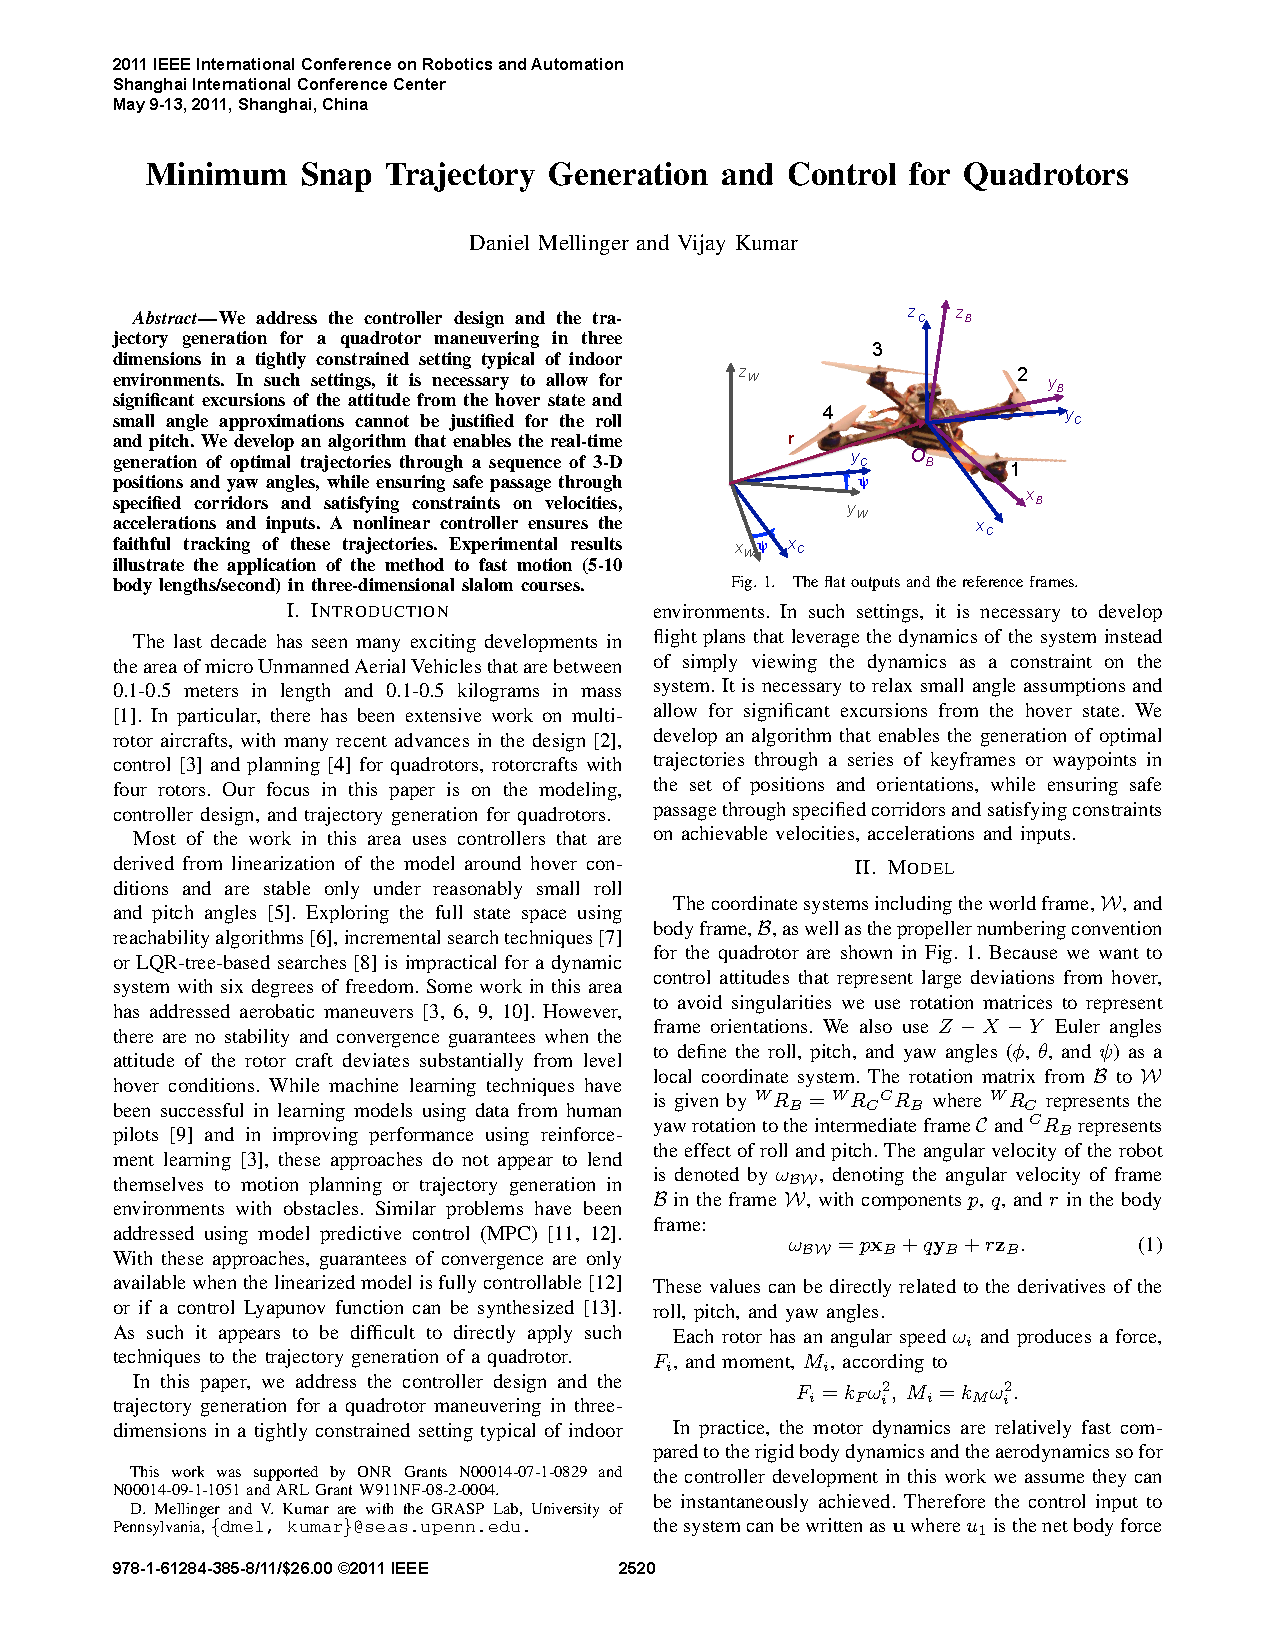
\includepdf[pages=-,scale=.8,pagecommand={}]{chap5_trajectory_planning/papers/MellingerKumar11.pdf}


%----------------------------------
\section{Path Planning using a Digital Elevation Map}

Add a discussion similar to this paper.

cite{ManyamCasbeerWeintraub21}:  This paper uses a delaney trangulation to parameterize the free space, and then moves control points within the delayney triangles to satisfy constraints.


%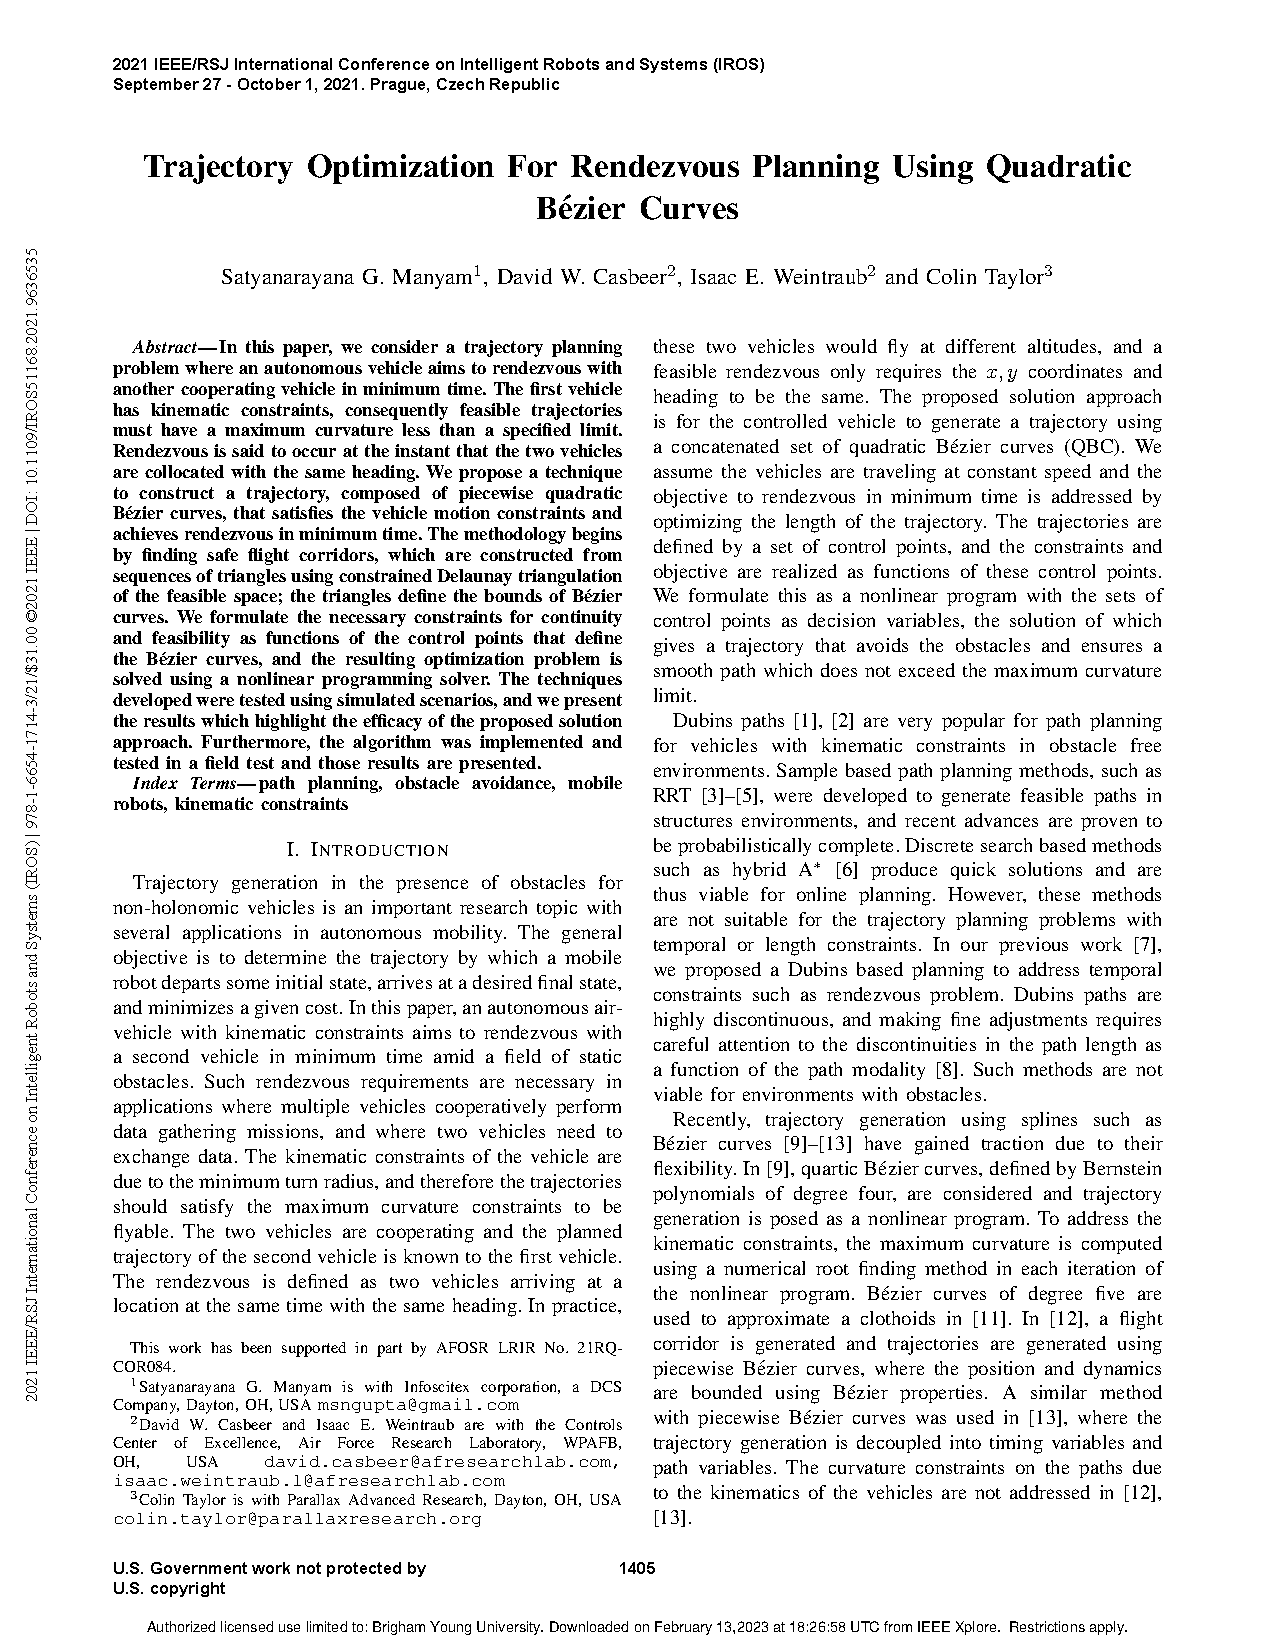
\includepdf[pages=-,scale=.8,pagecommand={}]{chap5_trajectory_planning/papers/ManyamCasbeerWeintraub21.pdf}

\cite{GaoWuLin18}:  This paper gets a quick and dirty path using the fast marching method, and then creates boxes around the desired trajectory produces a safe path corridor.  The b-spline paths are then optimized to stay within the corridor.
%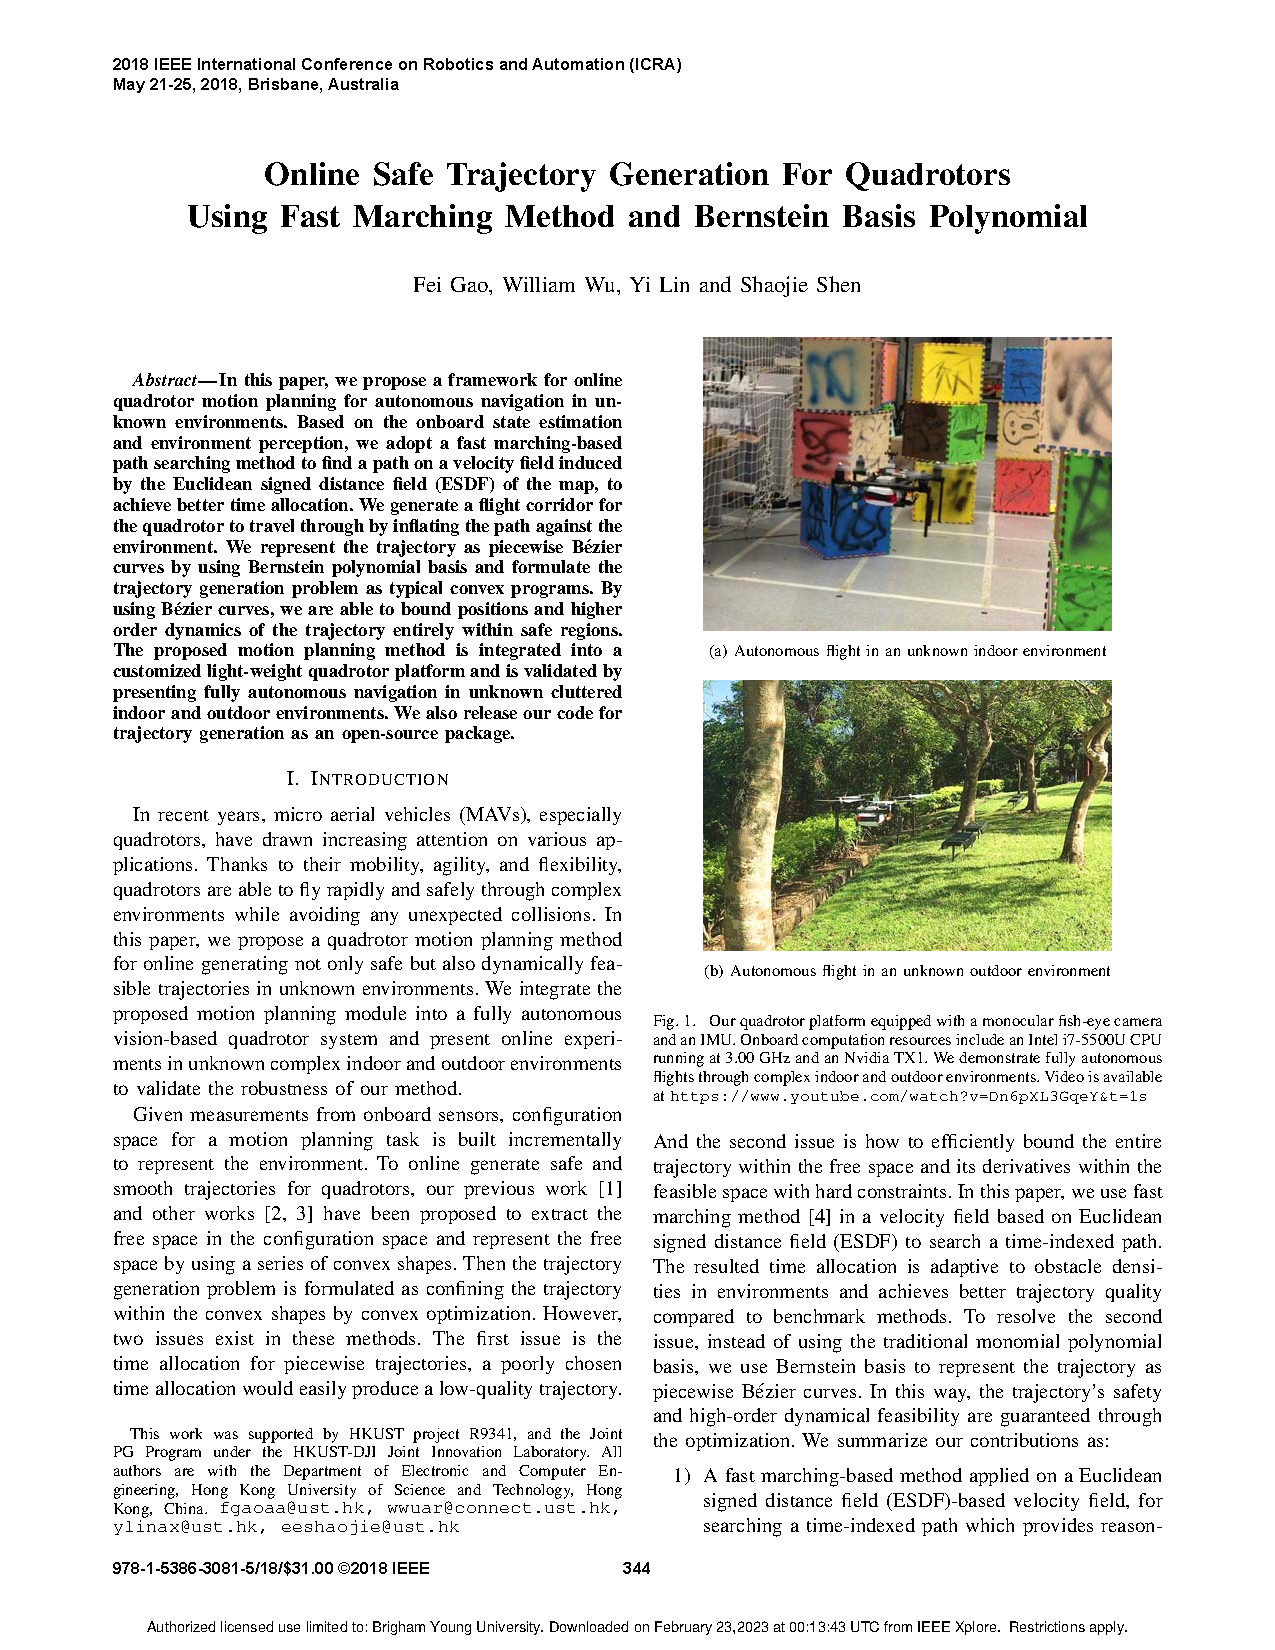
\includepdf[pages=-,scale=.8,pagecommand={}]{chap5_trajectory_planning/papers/GaoWuLin18.pdf}


\cite{PetresPailhasPatron}:  This paper shows how to get quick and dirty paths using the Fast Marching Method (FMM).

%\includepdf[pages=-,scale=.8,pagecommand={}]{chap5_trajectory_planning/papers/PetresPailhasPatron.pdf}


\cite{LutzMeurer21}:  Collision avoidance constraints, as describe in~\cite{LutzMeurer21}.
If the obstacles are ellipsoids:  Suppose that the world is modeled by a set of ellipsoidal obstacles
\[
\mathcal{O}_i = \{x\in\mathbf{R}^3: x^\top P_i x \leq 1\}
\]
and the total set of obstacles in the world is 
\[
\mathcal{W} = \bigcup_{i=1}^{M} \mathcal{O}_i.
\]
In this case, we want to ensure that none of the control points is in an obstacle, i.e., that

This paper shows how to formulate the obstacle avoidance problem as a convex problem using dual variables.
%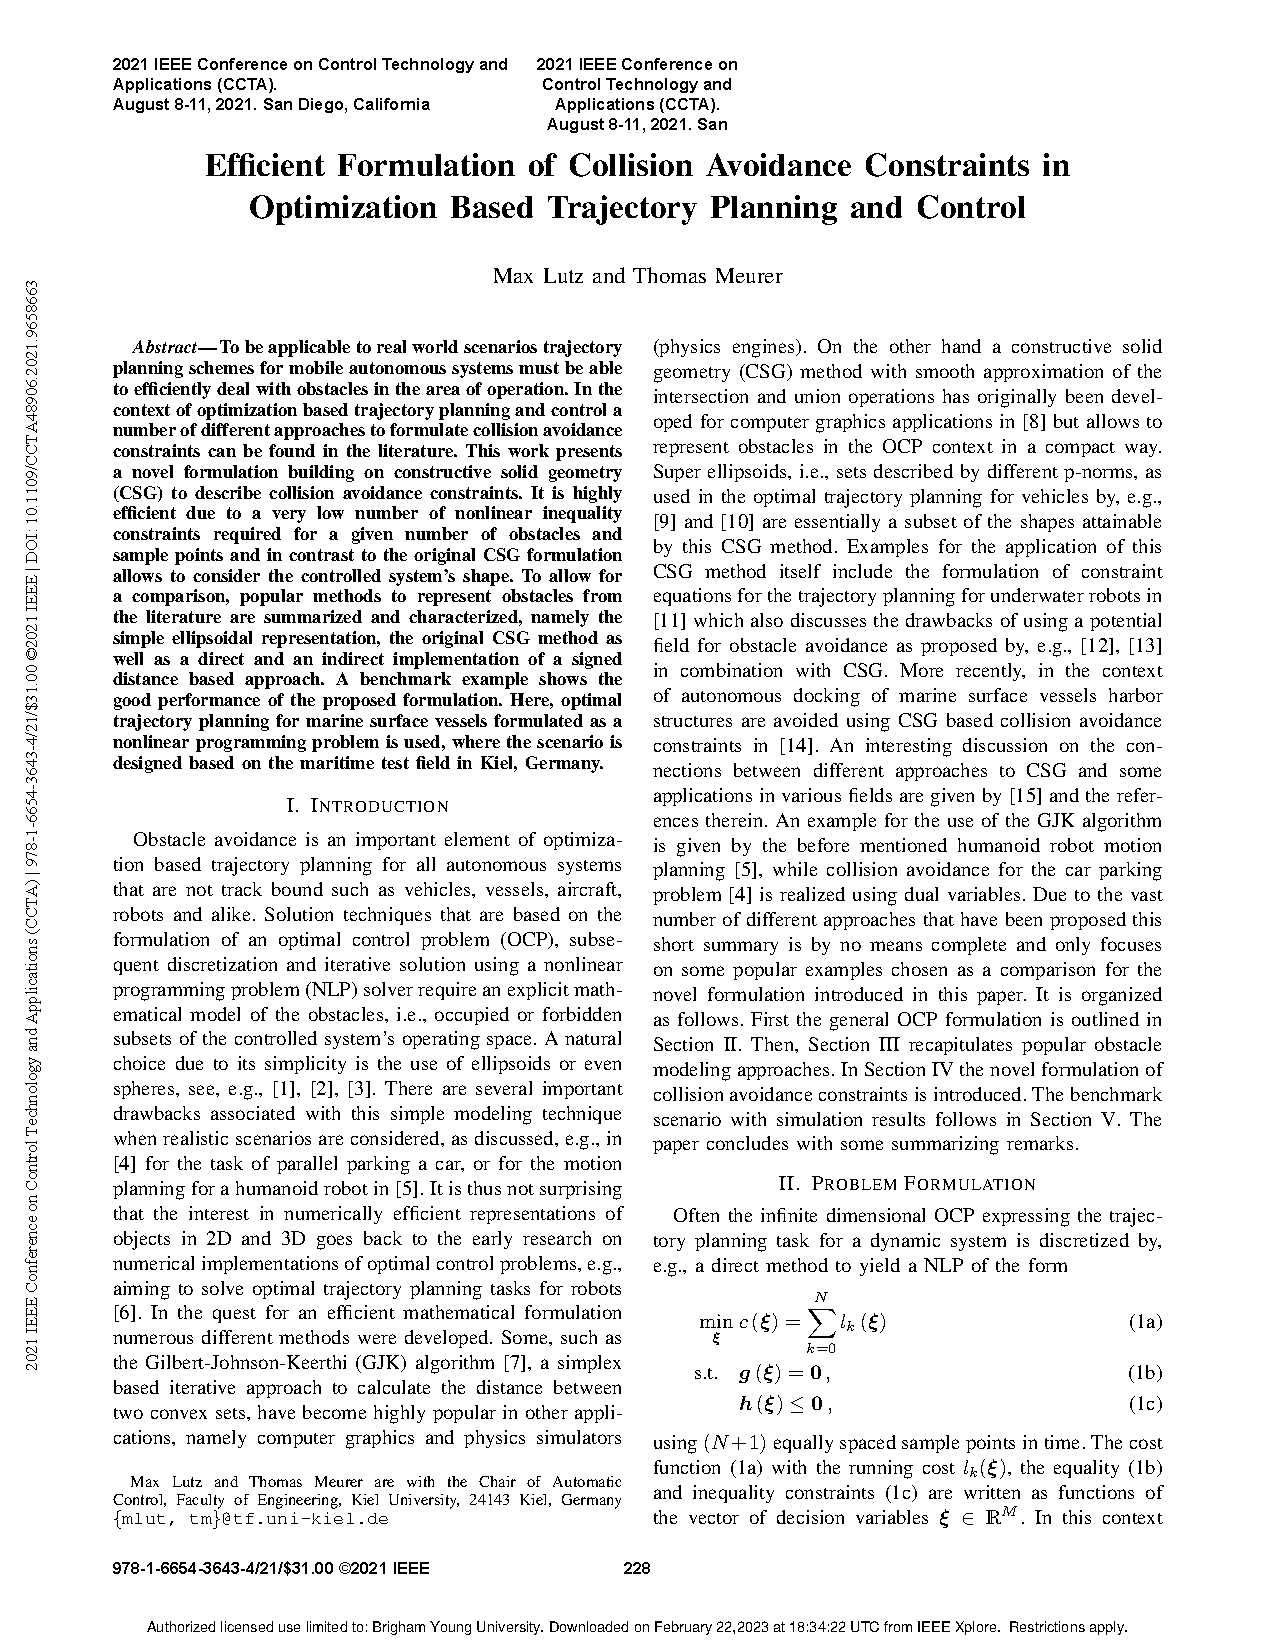
\includepdf[pages=-,scale=.8,pagecommand={}]{chap5_trajectory_planning/papers/LutzMeurer21.pdf}





%%----------------------------------
%\section{Voxel map}
%
%\rwbcomment{Add Thane's stuff here.}
%
%\subsection{OctoMaps}
%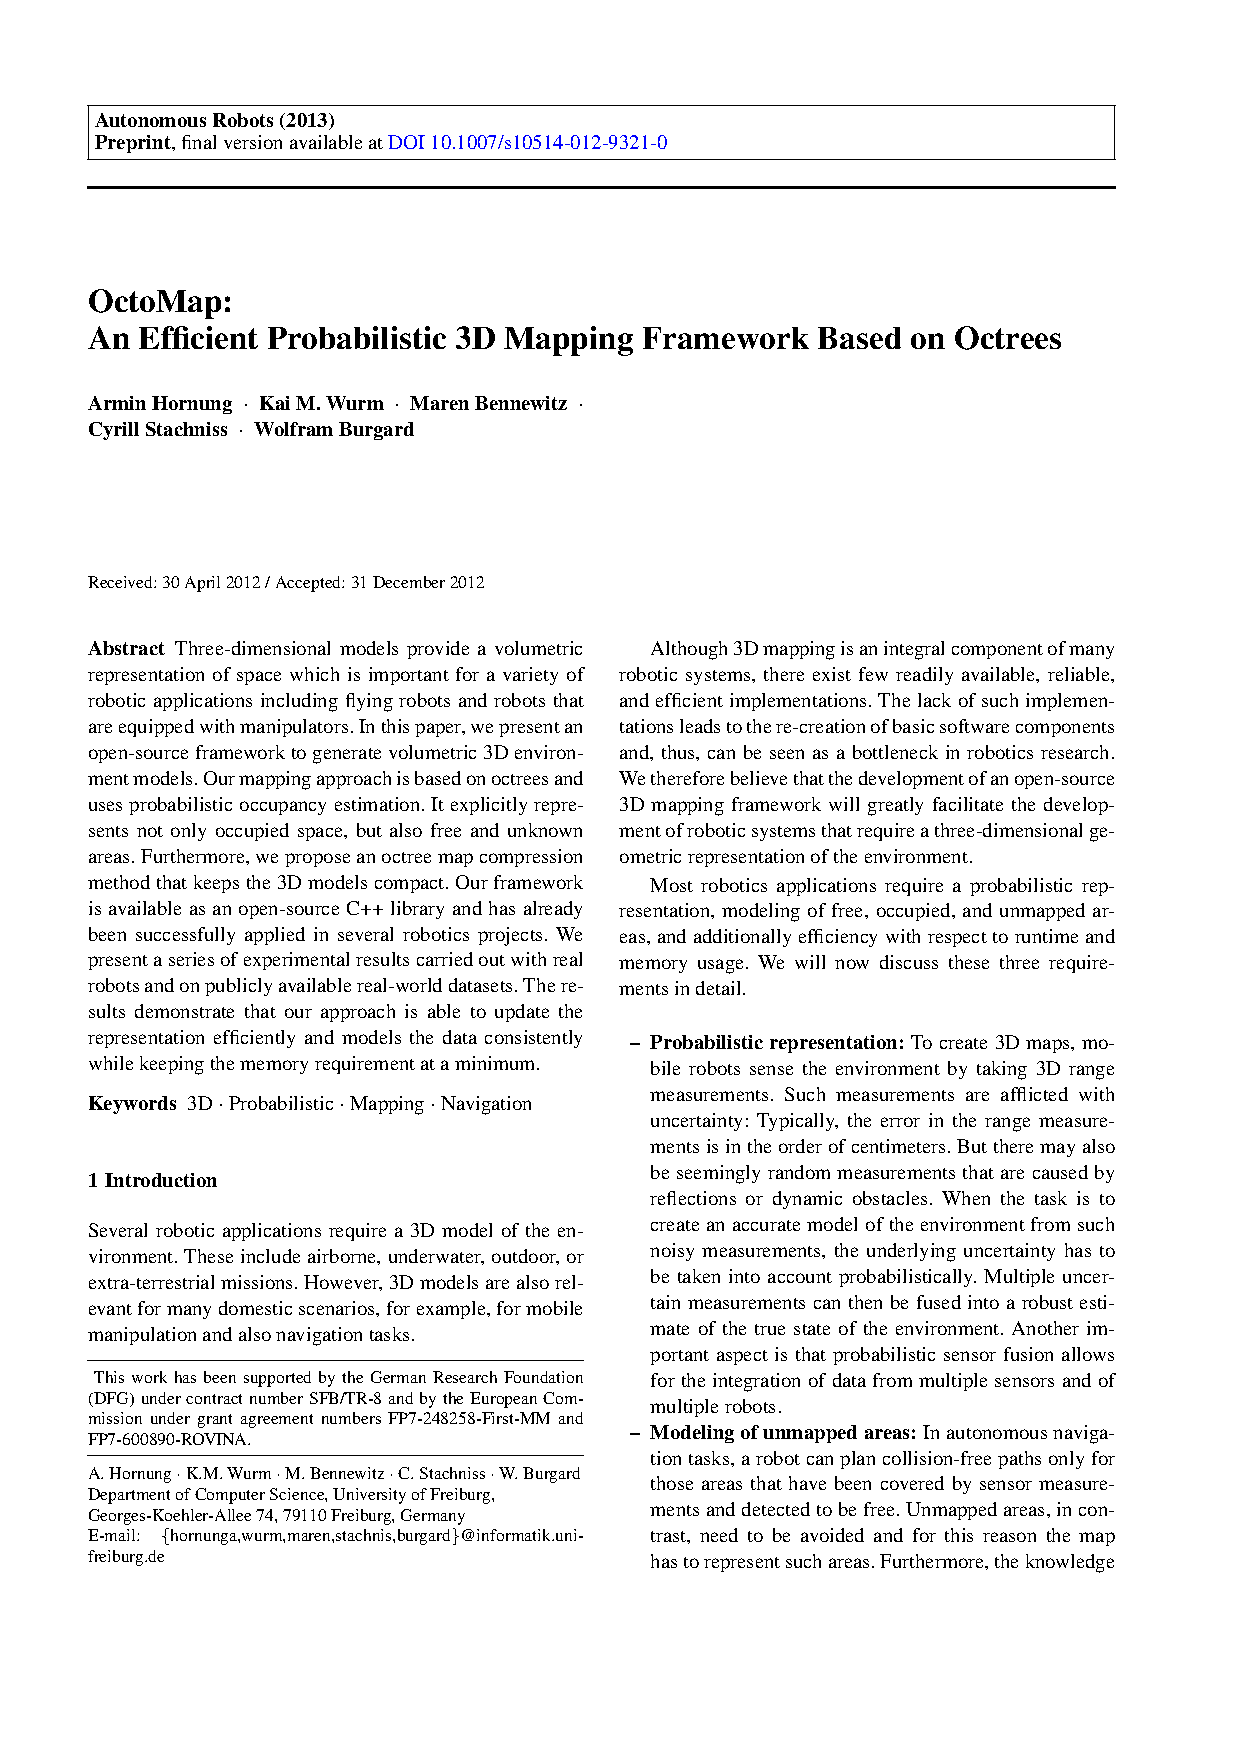
\includepdf[pages=-,scale=.8,pagecommand={}]{chap5_trajectory_planning/papers/Octomap.pdf}


%%----------------------------------
%\section{Waypoint planning in a voxel map}
%
%\subsection{Graph searching methods}
%%
%\begin{marginfigure}
%  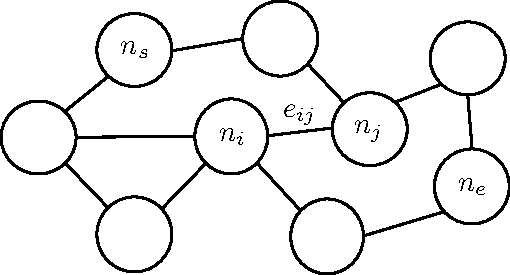
\includegraphics[width=\linewidth]{chap5_trajectory_planning/figures/plan-graph}
%  \caption{General graph structure for path planning.}
%  \label{fig:plan-graph}  
%\end{marginfigure}
%%
%We can model our world efficiently using discrete graphs where the nodes of the graph represent locations and the edges represent paths between locations. Typically we associate a cost with traveling along an edge from one node to the next. Figure~\ref{fig:plan-graph} shows a simple graph with a start node $n_s$, an end node $n_e$, and intermediate nodes $n_i$ and $n_j$. The cost for traveling along the edge from node $n_i$ to node $n_j$ is given by $e_{ij}$. Although not labeled, each edge has an associated cost. Edges can be unidirectional or bidirectional with with a uniform or different edge cost for each traversal direction. Edge costs can be used to represent proximity to obstacles, the physical distance between the two nodes, or other features of the environment. 
%
%The voxel maps described in the prior section can be represented as a graph structure where the center of the voxel is the node and cost for moving between adjacent voxels is the associated edge cost. To plan paths from a starting location in the voxel map to the specified goal location, we will utilize graph searching methods including widely used approaches such as Djikstra's algorithm and A* search.
%
%\vspace{1.0in}
%
%\rwbcomment{Add something like the following:}
%
%\href{https://www.redblobgames.com/pathfinding/a-star/introduction.html}{Introduction to A*}
%\href{https://brilliant.org/wiki/dijkstras-short-path-finder/}{Dijkstra's Algorithm}




